%%%%%%%%%%%%%%%%%%%%%%%%%%%%%%%%%%%%%%%%%
% American Geophysical Union (AGU)
% LaTeX Template
% Version 1.0 (3/6/13)
%
% This template has been downloaded from:
% http://www.LaTeXTemplates.com
%
% Original author:
% The AGUTeX class and agu-ps referencing style were created and are owned
% by AGU: http://publications.agu.org/author-resource-center/author-guide/latex-formatting-toolkit/
%
% This template has been modified from the blank AGU template to include
% examples of how to insert content and drastically change commenting. The
% structural integrity is maintained as in the original blank template.
%
% Important notes:
% This template retains extensive commenting from the AGU template. It is heavily
% advised you read these comments and follow them in order to insure a speedy
% submission process.
%
%%%%%%%%%%%%%%%%%%%%%%%%%%%%%%%%%%%%%%%%%

%%%%%%%%%%%%%%%%%%%%%%%%%%%%%%%%%%%%%%%%%%%%%%%%%%%%%%%%%%%%%%%%%%%%%%%%%%%%
% AGUtmpl.tex: this template file is for articles formatted with LaTeX2e,
% Modified March 2013
%
% This template includes commands and instructions
% given in the order necessary to produce a final output that will
% satisfy AGU requirements.
%
% PLEASE DO NOT USE YOUR OWN MACROS
% DO NOT USE \newcommand, \renewcommand, or \def.
%
% FOR FIGURES, DO NOT USE \psfrag or \subfigure.
%
%%%%%%%%%%%%%%%%%%%%%%%%%%%%%%%%%%%%%%%%%%%%%%%%%%%%%%%%%%%%%%%%%%%%%%%%%%%%
%
% All questions should be e-mailed to latex@agu.org.
%
%%%%%%%%%%%%%%%%%%%%%%%%%%%%%%%%%%%%%%%%%%%%%%%%%%%%%%%%%%%%%%%%%%%%%%%%%%%%

% Step 1: Set the \documentclass

% There are two options for article format: two column (default) and draft.

% PLEASE USE THE DRAFT OPTION TO SUBMIT YOUR PAPERS.
% The draft option produces double spaced output.

% Choose the journal abbreviation for the journal you are submitting to:

% jgrga	JOURNAL OF GEOPHYSICAL RESEARCH
% gbc	GLOBAL BIOCHEMICAL CYCLES
% grl		GEOPHYSICAL RESEARCH LETTERS
% pal	PALEOCEANOGRAPHY
% ras	RADIO SCIENCE
% rog	REVIEWS OF GEOPHYSICS
% tec	TECTONICS
% wrr	WATER RESOURCES RESEARCH
% gc		GEOCHEMISTRY, GEOPHYSICS, GEOSYSTEMS
% sw	SPACE WEATHER
% ms	JAMES
%
%
%
% (If you are submitting to a journal other than jgrga,
% substitute the initials of the journal for "jgrga" below.)

\documentclass[draft, jgrga]{AGUTeX}

% can I use these symbols?
\usepackage{array,amssymb}

% permil symbol
\usepackage{ wasysym }

% To create numbered lines:

% If you don't already have lineno.sty, you can download it from http://www.ctan.org/tex-archive/macros/latex/contrib/ednotes/ (or search the internet for lineno.sty ctan), available at TeX Archive Network (CTAN). Take care that you always use the latest version.

% To activate the commands, uncomment \usepackage{lineno} and \linenumbers*[1]command, below:

%\usepackage{lineno}
%\linenumbers*[1]

%  To add line numbers to lines with equations:
%  \begin{linenomath*}
%  \begin{equation}
%  \end{equation}
%  \end{linenomath*}

%%%%%%%%%%%%%%%%%%%%%%%%%%%%%%%%%%%%%%%%%%%%%%%%%%%%%%%%%%%%%%%%%%%%%%%%%
% Figures and Tables

% DO NOT USE \psfrag or \subfigure commands.

%  Figures and tables should be placed AT THE END OF THE ARTICLE, after the references.

%  Uncomment the following command to include .eps files (comment out this line for draft format):
%\usepackage[dvips]{graphicx}
\usepackage{graphicx}
\usepackage{caption}
%\usepackage{subfig}


% Substitute one of the following for [dvips] above if you are using a different driver program and want to proof your illustrations on your machine:
% [xdvi], [dvipdf], [dvipsone], [dviwindo], [emtex], [dviwin],
% [pctexps],  [pctexwin],  [pctexhp],  [pctex32], [truetex], [tcidvi],
% [oztex], [textures]

%  Uncomment the following command to allow illustrations to print when using Draft:
\setkeys{Gin}{draft=false}

% See how to enter figures and tables at the end of the article, after references.

%----------------------------------------------------------------------------------------
%	RUNNING HEAD AND CORRESPONDING AUTHOR
%----------------------------------------------------------------------------------------

% Author names in capital letters:
\authorrunninghead{Authors}

%------------------------------------------------

% Shorter version of title entered in capital letters:
\titlerunninghead{ESTIMATING DIFFUSION LENGTH}

%------------------------------------------------

% Corresponding author mailing address and e-mail address:
\authoraddr{Corresponding author: Emma C. Kahle, Earth and Space Sciences Department, University of Washington, Seattle, WA, USA. (eckahle@uw.edu)}

%----------------------------------------------------------------------------------------

\begin{document}

%----------------------------------------------------------------------------------------
%	TITLE
%----------------------------------------------------------------------------------------

\title{A Generalized Approach to Estimating Diffusion Length of Stable Water Isotopes from Ice Core Data}

%----------------------------------------------------------------------------------------
%	AUTHORS AND AFFILIATIONS
%----------------------------------------------------------------------------------------

% Use \author{\altaffilmark{}} and \altaffiltext{}

% \altaffilmark will produce footnote; matching \altaffiltext will appear at bottom of page.

\authors{Emma C. Kahle,\altaffilmark{1}
Christian Holme,\altaffilmark{2} Tyler R. Jones,\altaffilmark{3}  Vasileios Gkinis,\altaffilmark{2}} and Eric J. Steig\altaffilmark{1}

\altaffiltext{1}{Department of Earth and Space Sciences, University of Washington, Seattle, Washington, USA.}

\altaffiltext{2}{The Niels Bohr Institute, Centre for Ice and Climate, Juliane Maries Vej 30, 2100 Copenhagen, Denmark}

\altaffiltext{3}{Institute of Arctic and Alpine Research, University of Colorado, Boulder, CO 80309-0450, USA}

%----------------------------------------------------------------------------------------
%	ABSTRACT
%----------------------------------------------------------------------------------------

% Do NOT include any \begin...\end commands within the body of the abstract.

\begin{abstract}

Diffusion of water vapor in the porous firn layer of polar ice sheets causes the damping of high-frequency variations in water-isotope ratios. Spectral analysis of water isotope profiles from ice cores to determine characteristic firn-diffusion lengths can provide information about firn conditions in the past. High-resolution water isotope data were obtained by continuous flow analysis (CFA) from ice cores from the West Antarctic Ice Sheet Divide and the South Pole. The spectra of CFA data from these cores show different characteristics than the spectra of data obtained from measurements of discrete ice-core samples.  The higher resolution and greater signal to noise ratio of CFA data, compared to discrete data, affects the estimation of diffusion lengths. Two new diffusion-length estimation techniques are proposed, which can be applied to both CFA and discretely-sampled data. We evaluate these techniques and discuss possible influences of the CFA system on the continuously-measured data.

\end{abstract}

%----------------------------------------------------------------------------------------
%	ARTICLE CONTENT
%----------------------------------------------------------------------------------------

% The body of the article must start with a \begin{article} command
% \end{article} must follow the references section, before the figures and tables.

\begin{article}

\section{Introduction}

Water isotope data from ice cores have long been used as climate proxies, based on the temperature-dependent distillation of water isotope ratios (e.g. $\delta^{18}$O) in the atmosphere \citep{Epstein1951,Dansgaard1954,Dansgaard1964}. This traditional method for obtaining past temperature relies on empirical correlations that only approximate the physical processes involved. An alternative approach uses the signal of isotope diffusion preserved in the ice as a proxy for past site temperature \citep{Johnsen2000}.

Water isotope diffusion occurs primarily in the firn layer, snowfall in the upper tens of meters of an ice sheet that has yet to be fully compressed into ice. Because firn is permeable, water molecules can diffuse in the vapor phase, damping the seasonal variations and high-frequency noise of the original isotope signal. Because the diffusion process depends on temperature, a temperature record can be obtained by determining the extent of diffusion that has occurred, quantified as a ``diffusion length" \citep{Johnsen2000}. This method is independent of conventional assumptions about isotope fractionation before deposition, and thus has the potential to improve upon on conventional ice core paleotemperature methods. Diffusion estimates also provide constraints on past firn conditions and ice thinning history.

With these motivations, estimates of diffusion length have been made for ice cores in both Greenland and Antarctica \citep{Simonsen2011,Gkinis2014,vanderWel2015,Jones2017a,Holme2017}. Most estimates have used spectral analysis, as originally suggested by \citet{Johnsen1977}, to determine the degree to which high frequencies in the data have been damped. Existing methods for estimating diffusion do not work equally well for all data sets. In particular, high-resolution isotope data obtained using recently-developed continuous-flow measurement systems have somewhat different spectral characteristics than those obtained by measurements of discrete ice samples \citep{Jones2017a}. This difference complicates the estimation of diffusion lengths. In this paper we describe two general approaches to determine diffusion length. We use new data as well as previously published data to demonstrate the effectiveness of these approaches on all data sets. We also discuss potential sources for these spectral differences in the continuously-measured data.

%------------------------------------------------

\section{Isotope Diffusion Theory}

The majority of water isotope diffusion occurs in the firn layer where interconnected air pathways allow water vapor to diffuse vertically through the firn column. After firn densification has sealed off bubbles in the ice, vapor diffusion ceases and only solid ice diffusion continues. The process in solid ice has a diffusivity orders of magnitude smaller than that of vapor diffusion, and we do not consider it in this study.

The isotope profile in the firn layer of an ice sheet changes both due to diffusion across isotopic gradients and due to densification of the firn. These changes to the isotopic profile can be described by Fick's second law, the basic advection-diffusion equation:
\begin{equation}
\frac{\partial \delta}{\partial t}
= D \frac{\partial ^2 \delta}{\partial z^2}
- \dot{\epsilon}
z \frac{\partial \delta}{\partial z},
\end{equation}
where $\delta$ is the isotope ratio, $D$ is the diffusivity coefficient, $z$ is the vertical coordinate assuming an origin fixed on a sinking layer of firn, and $\dot{\epsilon}$ is the vertical strain rate \citep{Johnsen1977, Whillans1985}. The term $\dot{\epsilon} z$ can be thought of as the vertical velocity.

As shown by \citet{Johnsen1977} and subsequently used in many diffusion studies \citep{Cuffey1998, Whillans1985, Johnsen2000, Simonsen2011, Gkinis2014, vanderWel2015, Jones2017a, Holme2017}, a solution for the isotopic profile at time $t$ and depth $z$ in the firn column is given by:
\begin{equation}
\label{eq:diff_sol}
\delta (z,t) = S(t) \frac{1}{\sigma \sqrt{2 \pi}}
\int^\infty_{-\infty} \delta (z,0) \exp \left(\frac{-(z-u)^2}{2 \sigma ^2} \right)du,
\end{equation}
where $S(t)$ is the total thinning the layer has experienced due to ice flow from $t=0$ to $t=t'$:
\begin{equation}
S(t') = \exp \left( \int^{t'}_{0} \dot{\epsilon}(t) dt \right),
\end{equation}
and $\sigma$ is the ``diffusion length." The diffusion length quantifies the average vertical displacement of water molecules (excluding the advection) before they reach the bottom of the firn.

Equation \ref{eq:diff_sol} is the convolution of the initial isotope profile, $\delta(z,0)$, with a Gaussian filter of standard deviation equal to the diffusion length $\sigma$ \citep{Johnsen2000}:
\begin{equation}
\mathcal{G} = \frac{1}{\sigma \sqrt{2\pi}} \exp \left( \frac{-z^2}{2\sigma^2} \right).
\end{equation}

To solve this convolution, we take the Fourier transform of both sides of the equation:
\begin{equation}
  \delta(z,t) = \delta(z,0)*\mathcal{G} \qquad \Rightarrow \qquad \hat{\delta}(z,t) = \hat{\delta}(z,0) \cdot \hat{\mathcal{G}},
\end{equation}
where $*$ represents the convolution and \quad $\hat{}$ \quad represents the Fourier transform. The Fourier transform of a Gaussian remains a Gaussian:
\begin{equation}
  \label{eq:guass_fit}
\mathfrak{F}(\mathcal{G}) = \hat{\mathcal{G}} = \exp \left( \frac{-k^2\sigma^2}{2} \right),
\end{equation}
where $k$ is wavenumber. Equation \ref{eq:guass_fit} represents the ideal exponential model for diffusion. One can solve for $\sigma$ by optimizing the fit between Equation \ref{eq:guass_fit} and the power spectral density of the isotope data. Repeating this method over consecutive windowed sections of data yields diffusion length estimates through the length of an ice core.

%------------------------------------------------

\section{Water Isotope Data}

For most ice cores, water isotope data have been measured discretely by melting vertical sections of the core to produce a sample. The isotope ratio of each discrete sample is measured by mass spectrometry or laser spectroscopy \citep{Kerstel1999, Lis2008, Gupta2009, Brand2009}. More recently, ice core water-isotope measurements have been measured on continuous flow analysis (CFA) systems. CFA systems continuously feed the water isotopes of the melting core into a laser spectrometer, yielding high resolution data \citep{Gkinis2011a,Emanuelsson2015,Jones2017b}. The sample travels through a series of tubing, passing through a filter unit and vaporizer before entering the spectrometer. For more thorough information on the CFA set up used to measure the data in this paper, see \citet{Jones2017b}. Depending on the amount of effort committed, discrete analyses can produce resolutions ranging from $\sim$1/2 meter for entire ice cores to $\sim$1 cm for smaller sections of ice cores. CFA systems have been used to produce results with an effective resolution of 1/2 cm for an entire ice core record.

\subsection{Water Isotope Datasets}
In this paper, we use previously-published data from the WAIS Divide ice core (WDC) \citep{Jones2017b} and sections of data from a new ice core at the South Pole (SPC). Details of the SPC ice core project are given in \citet{Casey2014}. Both the WDC and SPC ice cores were measured continuously at the Institute of Arctic and Alpine Research (INSTAAR) at the University of Colorado and cross-calibrated by discrete measurements at the University of Washington IsoLab. For WDC, a Picarro L2130-\textit{i} laser spectrometer was used for $\delta^{18}$O and $\delta$D measurements; details are given in \citet{Jones2017b}.  For SPC, we built off the system used for WDC, adding a Picarro L2140-\textit{i} \citep{Steig2014} to the CFA system to additionally obtain measurements of $\delta^{17}$O. We use the first 2800 meters of WDC, corresponding to approximately the last 30,000 years. As of this writing, the full SPC record is still being processed; we use two 50-meter sections, one from the early Holocene and one from the last glacial period. For comparison we also use other published discrete and continuous water isotope datasets from Greenland and Antarctic ice cores presented in \citet{Oerter2004,Gkinis2011a,Steig2013,Svensson2015,Holme2017}.

\subsection{Power Spectra of Water Isotope Data Windows}
To calculate the power spectral density of these data sets, we use Burg's spectral analysis method and assume a 1-order autoregressive process. Figure \ref{spectra_disVScfa} compares the resulting spectra, normalized to unit power spectral density at the lowest frequency. We follow the methods used in \citet{Gkinis2014} to minimize the misfit in a least squares sense between the power spectral density of the data and a model, which follows from Equation \ref{eq:guass_fit}, given by the following:

\begin{equation}
  \label{exp_model}
  P_\sigma=P_0e^{-k^2\sigma^2}
\end{equation}

where $P_0$ is the original power level before the damping due to diffusion. A key assumption made in this procedure is that any variations in frequency in the power spectrum of the surface snow are small compared to the damping of high frequencies due to diffusion. \citep{Gkinis2014} justified this assumpition.

Furthermore, the right panel of Figure \ref{spectra_disVScfa} demonstrates the evolution of CFA measurements through time, which provides insight into how the CFA system affects the power spectrum of the data. These effects arise from improvements to the Picarro instruments and associated software combined with changes in the CFA system melt rate. This result is due to the averaging of raw data to an even depth scale prior to calculation of the spectrum. Raw data from each continuously-measured core is averaged to an even depth scale of 1/2 cm. Since each core is measured with a particular ice core melt rate and instrument data aquistion rate, the dataset from each core averages over a different number of raw points in sampling to the 1/2 cm scale. Averaging over more data points at each sampled depth produces a smoother dataset with further-damped high frequencies, and thus the data spectra from each core have varying high-frequency noise levels. Table \ref{tab:picarro_table} summarizes the instruments and sampling protocols used for each ice core measurement. In general, as instruments and CFA systems have improved, the baseline noise level of the power spectra have dropped.


%------------------------------------------------

\section{Previous Methods of Estimating Diffusion Length from Data}

Previous methods of estimating diffusion length have been effectively used for discretely-sampled data in a number of studies \citep{Johnsen2000,Simonsen2011,Gkinis2014,vanderWel2015}. These methods also work well with spectra from theoretically-derived synthetic data \citep{Holme2017}. Based on the exponential model in Equation \ref{exp_model}, these methods are effective because the spectra of these discretely-measured and synthetically-created data follow the exponential behavior closely. However, these diffusion estimation methods cannot be applied to spectra from continuously-measured data because these spectra deviate from the exponential model, with power decaying more slowly toward higher frequencies (from $10-40$ cycles/m or from periods of approximately $2.5-10$ cm of ice). Figure \ref{spectra_disVScfa} demonstrates this difference between the spectra of discretely- and continuously-measured data. This type of behavior can likely be explained by memory processes within the CFA system; we expand on these ideas in the Discussion.  This section describes some of these previous methods and demonstrates the need for more general techniques that can also be applied to continuously-measured data.

To estimate the extent of diffusion that occurred in the firn, the spectral power added from the measurement process must be separated from the firn diffusion signal. Each method separates the firn diffusion signal in a different way. One approach to this separation is to measure the differential diffusion, the difference between diffusion lengths of each isotope. The added measurement noise is the same for each isotope and is canceled out in the differential diffusion length. However, \citet{Holme2017} showed that differential diffusion methods are less precise and less accurate than single-isotope diffusion when converting to temperature. Thus we focus only on the single-isotope diffusion methods in this paper.

A method for estimating diffusion length from a single isotope is given in \citet{Gkinis2014}, which mathematically isolates the diffusion signal from the measurement noise. This technique uses a parameterization of the data that separates the firn diffusion signal from the instrument noise. The parameterization is fit to windowed sections of the data using a least-squares optimization by varying four parameters. The parameterization $P_s$ is the sum of two functions:

\begin{equation}
P_s =    P_0 {e}^{-k^2 \sigma^2} + \frac{\varsigma_{\mathrm{\eta}}^2 \Delta}
{\left| 1-a_1 \exp{\left( -i k  \Delta \right) } \right|^2},
\label{eq:powerspectrum}
\end{equation}
where the varied parameters are $a_1$, the AR-1 coefficient; $\varsigma_{\mathrm{\eta}}^2$, the variance of the noise; and $\frac{1}{\Delta}$, the sampling frequency. The first function is a Gaussian, the exponential model representing the high-frequency damping of firn diffusion, and the second function is an autoregressive noise signal of order 1 (AR-1), representing noise added from the measurement process. The parameters are allowed to vary within bounds that are wide enough not to restrict the least-squares fit, but narrow enough to keep each function on the corresponding part of the curve.

This two-function technique has been used effectively to estimate diffusion lengths on many discretely-measured data sets \citep{Gkinis2014,Holme2017}. When applying this technique to continuously-measured data, we find that the deviation from the exponential model in the continuous spectra affects the technique's ability to effectively fit the data. Figure \ref{GR_fits} illustrates this issue with examples from the WDC and SPC ice cores. The poor total fit of the two-function model to the data spectrum affects the estimation of diffusion length.

\citet{Jones2017a} developed a method specifically for continuously-measured data that avoids this issue. This technique identifies the frequency at which the spectrum deviates from the exponential model and only includes lower frequencies in the Gaussian fit, cutting off higher frequencies. Figure \ref{cutoff} shows examples of this cut-off technique for data sections from WDC and SPC. This technique relies on the assumption that enough of the diffusion signal is preserved below the chosen cut-off frequency to result in a reliable diffusion estimate. This technique works well to avoid the issue of the deviation from the exponential model, but the technique relies on determining cut-off frequencies manually for each individual spectrum. A more efficient technique that works with continously-measured data is needed.

\section{Generalizing the Fitting Technique}
We consider two different approaches to a general fitting technique that works for continuous data and can also be applied to discrete data. The first approach masks the high-frequency deviation from the exponential model by adding white noise to the continuous data so that the two-function technique of \citet{Gkinis2014} can be effectively applied. The second approach builds on the two-function technique by including a third function in the parameterization that accounts for the slower decay of the continuous power spectra. In this section, each technique is introduced and illustrated on data sections from WDC and SPC.

\subsection{Technique 1: Adding White Noise}
The noise-adding technique masks the slow decay of the spectrum by adding noise to the signal, so that the two-function parameterization in Equation \ref{eq:powerspectrum} can be applied. We add normally-distributed noise to the data in the time domain, which increases the noise level in the frequency domain. With this added noise, the resulting power spectrum is much closer to the exponential model, and the two-function technique can now effectively fit the spectrum. Figure \ref{WAIS_spectrum_added_noise} illustrates this technique applied to a WDC data section. The disadvantage of this technique is that it manipulates the original signal and may mask useful information about climate.

We used a sensitivity test to optimize the magnitude of noise to add to the data. Adding too little noise does not effectively mask the deviation from the exponential model, but adding too much noise risks obscuring the climate signal. The test used a 500-year moving window throughout the WDC record. For each windowed section, 100 diffusion lengths were estimated by adding an increasing white noise baseline to the data in each window. A diffusion length was estimated for each tested noise level on each 500-year window. We defined the optimal noise level as that at which the diffusion length estimates stopped changing with increasing noise. This level can be found when the gradient of diffusion length with respect to added noise level approaches zero. Figure \ref{added_noise_sensitivity} shows how this gradient changes for both $\delta^{18}$O and $\delta$D throughout the WDC core. The optimal noise level is selected for each age as the lowest noise level that results in a gradient of approximately zero. For WDC, we found that the optimal added noise is Gaussian-distributed noise with a standard deviation of $0.4 \, \permil$ for $\delta^{18}$O and $3.0 \,\permil$ for $\delta$D.

\subsection{Technique 2: Parameterizing a Multi-Function Fit}
This technique creates a multi-function parameterization of the total spectrum by adding a third function to the two-function technique of \citet{Gkinis2014}. We tested three different functions as third terms in Equation \ref{eq:powerspectrum}, and we determined which addition yields the best full-spectrum fit. The three functions we tested were a second AR-1 function, a second Gaussian function, and a folded normal distribution (FND) \citep{Tsagris2014}:
\begin{equation}
\phi = \phi_{0} \cdot e^{-(k \cdot \psi)^2} \cdot |\left[1 - \Phi(-i k \psi)\right]|^2,
\end{equation}
where $\Phi(\psi) = 1/2\cdot \mathrm{erfc}(-\psi/2) $. Here $\phi_0$ and $\psi$ are the two parameters that are varied to optimize the fit. The justification of fitting a FND is that it reflects the unidirectional memory and diffusion induced by the one-way flow of the CFA system. A FND is the absolute value of a Gaussian distribution, resulting in a function that smooths in only one direction. Because water is continuously flowing in one direction through the CFA system, the application of a FND mimics this one-sided effect. We discuss these system effects further in the Discussion.

The results of these three parameterizations are shown in Figures \ref{GRR_fits} through \ref{folded_normal_gauss_spectrum} for WDC and SPC. Figure \ref{GRR_fits} shows the parameterization that sums a Gaussian curve and two autoregressive noise functions. With the inclusion of this third function in both WDC and SPC, the total fit is visually improved, as compared to the single-Gaussian fit in Figure \ref{GR_fits}, but still unable to effectively fit the spectrum, particularly for WDC. Figure \ref{GGR_fits} shows the parameterization that sums two Gaussian curves and one autoregressive noise function. Again there is a visual improvement in the total fit as compared to the single-Gaussian fit, now in both SPC and WDC. Finally, Figure \ref{folded_normal_gauss_spectrum} shows the parameterization that sums one Gaussian, one autoregressive noise function, and one FND function. Due to the close relationship between a Gaussian and a FND function, the fits in Figures \ref{GGR_fits} and \ref{folded_normal_gauss_spectrum} are very similar.

To describe the uncertainty of the diffusion length estimated by this approach, we use the 95th percent confidence bounds from the estimate of the power spectrum. The upper bound on diffusion length is found from combining the lowest frequencies of the upper power spectrum estimate with the highest frequencies of the lower power spectrum estimate. Figure \ref{uncertainty} demonstrates this approach, with dashed lines representing the upper and lower bounds on the fit of the parametrization. This approach produces a conservative estimate on the uncertainty associated with the estimate of diffusion length.

%------------------------------------------------

\section{Evaluating Fitting Techniques}
To evaluate each fitting technique, we compared the effectiveness of each method for the entire WDC record. First, we tested each technique based on how well it could fit the data spectra. We calculated the adjusted coefficient of determination ($\bar{r}^2$) as a metric of goodness of fit with the data. The coefficient of determination ($r^2$) is calculated by comparing the variability of the estimation errors with the variability of the original values. The adjusted coefficient of determination ($\bar{r}^2$) takes into account the number of variable parameters ($p$) as follows \citep{Theil1961}:
\begin{equation}
\bar{r}^2 = 1 - (1 -r^2) \frac{n - 1}{n - p - 1},
\end{equation}
where $n$ is the sample size. We use the $\bar{r}^2$ for this comparison because the techniques have different numbers of variable parameters (the noise-adding technique has five parameters, while the multi-function parameterizations each have six). Figure \ref{G_of_fit_1} plots the $\bar{r}^2$ values as a function of age for WDC. The $\bar{r}^2$ values of the double-Gaussian and FND parameterizations are indistinguishable, so we only include the double-Gaussian result. All the parameterizations provide good fits ($\bar{r}^2 > 0.9$) to the data, but the best fits are obtained with the double-Gaussian and FND parameterizations. For simplicity and computational efficiency, we prefer the double-Gaussian over the FND parameterization.

As a second means of evaluation, we compared the resulting diffusion length estimates for the double-Gaussian parameterization and noise-adding techniques. Figure \ref{WAIS_diffusion_adding_noise} shows the diffusion length estimates from both techniques plotted with respect to age. Both techniques reconstruct similar diffusion lengths, but the noise-adding method is more stable through the glacial period. This stability is attributed to the fact that, due to known measurement issues, the quality of some of the WDC data from the glacial period is poor. In this period, the water isotope signal contains several noisy sections of about half a meter. By adding white noise to the data, the noisy data sections are masked, making the fit more stable. However, as discussed above, masking noisy sections of the data may also mask useful climate information. Besides this stability issue in the glacial period, the two techniques match well throughout the record, bolstering confidence in their fitting abilities.

A third way of validating the results is by comparing their results with those of the cut-off technique presented in \citet{Jones2017a}. Since the cut-off technique results are not affected by the deviation from the exponential model, we can use them as a benchmark against which to validate these new techniques. Figure \ref{WAIS_diffusion_lengths} compares the two new techniques with the cut-off technique for the WDC record. The estimated diffusion lengths from this paper match within uncertainty bounds to those in \cite{Jones2017a}, again adding confidence to the validation of our techniques. As each of these techniques is indepedent of one another, the confidence bounds together provide insight into how well diffusion lengths can be estimated from ice core data currently. With the current state of our estimation abilities, we can clearly distinguish between Holocene and glacial diffusion lengths, but we must be careful when interpretting partiular peaks.

%------------------------------------------------

\section{Discussion}

\subsection{Automated Methods}
Through these evaluations, we conclude that the best technique for estimating diffusion length is the multi-function fit with the double-Gaussian parameterization, though the noise-adding method is also an option. While both methods produce reliable diffusion length results, we prefer the double-Gaussian parameterization because it does not alter the original signal. However, the noise-adding method may be useful if a water isotope dataset is noisy enough that the double-Gaussian fit cannot be used effectively.

These automated methods provide a more efficient approach to estimating diffusion length as compared to the manual cut-off method presented in \citet{Jones2017a}. However, each spectra must be checked manually to ensure the quality of each fit. Small alterations in the bounds of the parameters of the fit can improve the ability of the automated method the fit the entire spectrum. Furthermore, for a given ice core record, the general shape and magnitude of the spectra may shift with increasing depth of the data windows. Choosing sets of parameters for distinct regimes within the dataset (i.e. Holocene and Glacial) can improve the automated fit. While these manual checks require some amount of time, the total amount of time to produce diffusion length estimates through an entire ice core record is reduced as compared to using the fully-manual cut-off method.

\subsection{Spectral Effects of the CFA System}
While we have shown that these techniques effectively estimate the extent of firn diffusion, it remains unexplained why the spectra of continuously-measured data decay more slowly in the higher frequencies than the ideal exponential model. There are many possible sources of noise throughout the CFA measurement system that could affect the spectrum in this way. Mixing and memory effects are known to occur throughout the system as sample water travels to the instrument through tubing and various reservoirs \citep{Gkinis2011a}. For WDC, \citet{Jones2017b} ran mock ice of constant isotopic compositions through the CFA system. This procedure creates a step-change in isotopic value and characterizes the response of the system to isotopic changes. \citep{Jones2017b} showed how the system's response to this step-change can be estimated as a transfer function of the product of two lognormal CDFs:

\begin{equation}
  \label{transfer function}
  \delta_{model}(t) = \frac{1}{2}\left[1+erf\left(\frac{t-t_1}{\sigma_1\sqrt{2}}\right)\right] \cdot \frac{1}{2}\left[1+erf\left(\frac{t-t_2}{\sigma_2\sqrt{2}}\right)\right],
\end{equation}
where $t$ is time and $\sigma$ is the mixing length.

Through forward modeling of synthetically-diffused ice core data, we found that the shape of WDC power spectra can be simulated by using a system-smoothing process following this function (Figure \ref{smoothed_synthetic}). We estimated the parameters of Equation \ref{transfer function} by minimizing the fit between the WDC power spectrum and the spectrum of synthetic ice core data smoothed by Equation \ref{transfer function}. We checked this estimate by comparing the resulting transfer function with that calculated directly from the mock ice run through the CFA system. In this way, we found that the smoothing process of the system can be explained by this forward smoothing model. Inverting this model to find a function to use in the multi-function parameterization would be quite complicated. However, the FND function discussed in section 5.2 approximates well the diffusion physics that occur. We subsequently show that the double-Gaussian function gives indistinguishable results from the FND function, and thus we use the double-Gaussian parameterization to approximate the complex behavior of the above transfer function.

The CFA system response to isotopic changes characterizes the entire system, but we can also consider the response to isotopic changes within distinct parts of the system. For example, the Picarro laser spectrometer adds some amount of baseline noise to the data. Within the instrument, the water vapor sample is injected into a cavity where the isotopic composition is determined by measuring how quickly certain frequencies of a laser are absorbed by the sample. This measurement is affected by the amount of sample that remains in the cavity after most of it has been flushed out. Because there is a continuous stream of new sample vapor pumping into the cavity, the extent of this memory within the system will affect subsequent measurements. The timescales involved in this process can explain at least some of the spectral behavior seen in the continuously-measured data.

Additionally, we tested the consistency of the effects of the CFA system on the power spectrum. We measured replicate ice samples from the same depth of SPC (1060-1075m) and compared the resulting power spectra. Figure \ref{duplicate_spectra} plots blue and red curves, showing the power spectra from, respectively, the original and the replicate meaurements. The spectra do not differ significantly, suggesting that the effects of the CFA system on the spectra are consistent through time.

Figure \ref{duplicate_spectra} also isolates the effect of another distinct part of the CFA system. The yellow curve plots data that is the same as the red but that has been assigned slightly different depths at each point. As the CFA system melts the ice sample, a laser pointing down at the ice registers distance as the top surface moves downwards. This laser data must be processed to yield actual ice-core depths associated with each water isotope measurement. It is possible that this processing can produce spectral characteristics in the data. However, since the yellow curve does not differ from the red, we do not expect depth registration issues to significantly affect our ability apply automated fitting methods to the data measured and processed in this way.

These ideas give some insight into how the system is likely influencing the data spectrum. The full system smooths the data through mixing and memory processes. Distinct parts of the system such as the Picarro instrument contribute to this overall system effect. However, at this point we are unable to untangle all of the separate influences of different aspects of the system. Some parts of the system, like the laser depth registration and processing likely do not significantly affect the spectrum. The question as to the exact source or sources witin the CFA system of the deviation from the exponential model remains open.

%------------------------------------------------

\section{Conclusions}

In this study we examined the firn diffusion signal in continuously-measured water-isotope data from the WAIS Divide and South Pole ice cores. We observed that spectra from these CFA data, unlike spectra from comparable discretely-sampled data, have a different spectral behavior that deviates from the ideal exponential model. Previous diffusion-length estimate techniques fail to properly fit these continuous data due to this slower decay of power. We found that the most effective method to estimate diffusion lengths on these continuous data is the double-Gaussian parameterization of the multi-function fitting technique, while the noise-adding technique can be used as well. These methods are efficient in required time and effort and also effective in fitting the entire spectra of continuously-measured data. We validated the methods against one another as well as against results estimated independently by \citet{Jones2017a}. The exact cause of this spectral behavior within the CFA system remains an open question. However, these methods can be used to determine diffusion lengths on water isotope data from any ice core record of sufficiently high resolution. In the future, these methods will be used to estimates diffusion lengths on continuously-measured cores, including the entire SPC record.

%----------------------------------------------------------------------------------------
%	APPENDICES (OPTIONAL)
%----------------------------------------------------------------------------------------

%%%%%%%%%%%%%%%%%%%%%%%%%%%%%%%%
%% Optional Appendix goes here

% \appendix resets counters and redefines section heads
% but doesn't print anything.
% After typing  \appendix

% \section{Here Is Appendix Title}
% will show
% Appendix A: Here Is Appendix Title



% This statement requires citation \citep{AtkinsonSloan}. This one is an in-text citation because the authors of \citet{ColtonKress1} are specifically mentioned.

%\begin{equation}
%\label{eq:emc}
%e = mc^2
%\end{equation}

%Referencing equation \ref{eq:emc}

%Referencing table \ref{sampletable}

%Referencing Figure \ref{placeholder}

%\begin{eqnarray}
  %x_{1} & = & (x - x_{0}) \cos \Theta \nonumber \\
      %  && + (y - y_{0}) \sin \Theta  \nonumber \\
  %y_{1} & = & -(x - x_{0}) \sin \Theta \nonumber \\
      %  && + (y - y_{0}) \cos \Theta.
%\end{eqnarray}

%----------------------------------------------------------------------------------------
%	GLOSSARY OR NOTATION (OPTIONAL)
%----------------------------------------------------------------------------------------

%%%%%%%%%%%%%%%%%%%%%%%%%%%%%%%%%%%%%%%%%%%%%%%%%%%%%%%%%%%%%%%%
%
% Optional Glossary or Notation section, goes here
%
%%%%%%%%%%%%%%
% Glossary is only allowed in Reviews of Geophysics
% \section*{Glossary}
% \paragraph{Term}
% Term Definition here
%
%%%%%%%%%%%%%%
% Notation -- End each entry with a period.
% \begin{notation}
% Term & definition.\\
% Second term & second definition.\\
% \end{notation}
%%%%%%%%%%%%%%%%%%%%%%%%%%%%%%%%%%%%%%%%%%%%%%%%%%%%%%%%%%%%%%%%

%----------------------------------------------------------------------------------------
%	ACKNOWLEDGEMENTS
%----------------------------------------------------------------------------------------

\begin{acknowledgments}
The research leading to these results was funded by the National Science Foundation grant numbers 1443105 and 1443328 as well as from the European Research Council under the European Union's Seventh Framework Programme (FP7/2007-2013) grant agreement \#610055 as part of the ice2ice project.
\end{acknowledgments}

%----------------------------------------------------------------------------------------
%	BIBLIOGRAPHY
%----------------------------------------------------------------------------------------

% Either type in your references using
% \begin{thebibliography}{}
% \bibitem{}
% Text
% \end{thebibliography}

% Or,

% If you use BiBTeX for your references, please use the agufull08.bst file (available at % ftp://ftp.agu.org/journals/latex/journals/Manuscript-Preparation/) to produce your .bbl
% file and copy the contents into your paper here.

% Follow these steps:
% 1. Run LaTeX on your LaTeX file.

% 2. Make sure the bibliography style appears as \bibliographystyle{agufull08}. Run BiBTeX on your LaTeX
% file.

% 3. Open the new .bbl file containing the reference list and
%   copy all the contents into your LaTeX file here.

% 4. Comment out the old \bibliographystyle and \bibliography commands.

% 5. Run LaTeX on your new file before submitting.

% AGU does not want a .bib or a .bbl file. Please copy in the contents of your .bbl file here.

\begin{thebibliography}{}

\providecommand{\natexlab}[1]{#1}
\expandafter\ifx\csname urlstyle\endcsname\relax
  \providecommand{\doi}[1]{doi:\discretionary{}{}{}#1}\else
  \providecommand{\doi}{doi:\discretionary{}{}{}\begingroup
  \urlstyle{rm}\Url}\fi


\bibitem[{\textit{Brand et~al.}(2009)}]{Brand2009} Brand, W. A., Geilmann, H., Crosson, E. R., \& Rella, C. W. (2009), Cavity ring‐down spectroscopy versus high‐temperature conversion isotope ratio mass spectrometry; a case study on δ2H and δ18O of pure water samples and alcohol/water mixtures, \textit{Rapid Communications in Mass Spectrometry}, \textit{23}(12), 1879--1884.

\bibitem[{\textit{Casey et~al.}(2014)}]{Casey2014} Casey, K. A., Fudge, T. J., Neumann, T. A., Steig, E. J., Cavitte, M. G. P., and Blankenship, D. D. (2014), The 1500 m South Pole ice core: recovering a 40 ka environmental record, \textit{Annals of Glaciology}, \textit{55}(68), 137--146.

\bibitem[{\textit{Cuffey and Steig}(1998)}]{Cuffey1998}Cuffey, Kurt M. and Eric J. Steig. (1998), Isotopic diffusion in polar firn: implications for interpretation of seasonal climate parameters in ice-core records, with emphasis on central Greenland, \textit{Journal of Glaciology}, \textit{44.}(147), 273--284.

\bibitem[{\textit{Dansgaard}(1954)}]{Dansgaard1954} Dansgaard, W. (1954),
The $^{18}${O}-abundance in fresh water,
\textit{Geochimica et Cosmochimica Acta}, \textit{6}(5-6), 241--260.

\bibitem[{\textit{Dansgaard}(1964)}]{Dansgaard1964} Dansgaard, W. (1964),
Stable isotopes in precipitation,
\textit{Tellus B}, \textit{16}(4), 436--468.

\bibitem[{\textit{Dansgaard and Johnsen}(1969)}]{Dansgaard1969} Dansgaard, W. and S. J. Johnsen (1969), A flow model and a time scale for the ice core from Camp Century, Greenland, \textit{Journal of Glaciology}, \textit{8}(53), 215--223.

\bibitem[{\textit{Emanuelsson et~al.}(2015)}]{Emanuelsson2015}
Emanuelsson, B.~D., Baisden, W.~T., Bertler, N.~A.~N., Keller, E.~D. and V. Gkinis (2015),
High-resolution continuous-flow analysis setup for water isotopic measurement from ice cores using laser spectroscopy,
\textit{Atmospheric Measurement Techniques}, \textit{8}(7), 2869--2883.

\bibitem[{\textit{Epstein et~al.}(1951)}]{Epstein1951}
Epstein, S., Buchsbaum, R., Lowenstam, H. and H.C. Urey (1951),
Carbonate-water isotopic temperature scale,
\textit{Geological Society of America Bulletin}, \textit{62}(4), 417--426.

\bibitem[{\textit{Gkinis et~al.}(2011)}]{Gkinis2011a}
Gkinis, V., Popp, T.~J., Blunier, T., Bigler, M., Schupbach, S., Kettner, E. and S.~J. Johnsen (2011),
Water isotopic ratios from a continuously melted ice core sample,
\textit{Atmospheric Measurement Techniques}, \textit{4}(11), 2531--2542.

\bibitem[{\textit{Gkinis}(2011)}]{Gkinis2011b}
Gkinis, V. (2011),
{ High resolution water isotope data from ice cores},
PhD thesis, University of Copenhagen.

\bibitem[{\textit{Gkinis et~al.}(2014)}]{Gkinis2014}
Gkinis, V., Simonsen, S.~B., Buchardt, S.~L., White, J.~W.~C. and  B.~M. Vinther (2014),
{Water isotope diffusion rates from the NorthGRIP ice core for the last 16,000 years - glaciological and paleoclimatic implications},
\textit{Earth and Planetary Science Letters}, \textit{405}, 132--141.

\bibitem[{\textit{Gupta et~al.}(2009)}]{Gupta2009}
Gupta, P., Noone, D., Galewsky, J., Sweeney, C., \& Vaughn, B. H. (2009),
{Demonstration of high‐precision continuous measurements of water vapor isotopologues in laboratory and remote field deployments using wavelength‐scanned cavity ring‐down spectroscopy (WS‐CRDS) technology},
\textit{Rapid Communications in Mass Spectrometry}, \textit{23}(16), 2534--2542.

\bibitem[{\textit{Herron and Langway}(1980)}]{HerronLangway1980}
Herron, M., and Langway Jr, C. (1980). Firn densification: An empirical model. Journal of Glaciology, 25(93), 373-385.

\bibitem[{\textit{Holme et~al.}(2017)}]{Holme2017}
Holme, C., Gkinis, V., and B. M. ~Vinther (2017), Molecular
diffusion of stable water isotopes in polar firn as a proxy
for past temperatures, Under review in \textit{Geochimica et Cosmochimica Acta}.

\bibitem[{\textit{Jones et~al.}(2017a)}]{Jones2017a}
Jones, T.~R., Cuffey, K.~M., White, J.~W.~C., Steig, E.~J., Buizert, C.,
Markle, B.~R., McConnell, J.~R. and M. Sigl (2017a),
{Water isotope diffusion in the WAIS Divide ice core
	during the Holocene and last glacial},
\textit{J. Geophys. Res. Earth Surf.}, \textit{122}, 290–309.

\bibitem[{\textit{Jones et~al.}(2017b)}]{Jones2017b}
Jones, T.~R., White, J.~W.~C., Steig, E.~J., Vaughn, B.~H., Morris, V.,
Gkinis, V., Markle, B.~R. and S.~W. Schoenemann (2017b),
{Improved Methodologies for Continuous Flow Analysis of Stable
Water Isotopes in Ice Cores},
\textit{Atmos. Meas. Tech. Discuss}, \textit{10}, 617–-632.

\bibitem[{\textit{Johnsen}(1977)}]{Johnsen1977}
Johnsen, S.~J. (1977),
{Stable Isotope Homogenization of Polar Firn and Ice},
\textit{Isotopes and Impurities in Snow and Ice}, 201--219.

\bibitem[{\textit{Johnsen et~al.}(2000)}]{Johnsen2000}
Johnsen, S.~J., Clausen, H.~B., Cuffey, K.~M., Hoffmann, G., Schwander, J. and T. Creyts (2000),
{Diffusion of stable isotopes in polar firn and ice: the isotope effect in firn diffusion},
\textit{Physics of Ice Core Records}, 121--140.

\bibitem[{\textit{Kerstel et~al.}(1999)}]{Kerstel1999}
Kerstel, E. T., Van Trigt, R., Reuss, J., \& Meijer, H. A. J. (1999),
{Simultaneous determination of the 2H/1H, 17O/16O, and 18O/16O isotope abundance ratios in water by means of laser spectrometry},
\textit{Analytical Chemistry}, \textit{71}(23), 5297--5303.

\bibitem[{\textit{Lasaga}(2014)}]{Lasaga2014}
Lasaga, A. C. (2014),
{Kinetic theory in the earth sciences},
\textit{Princeton University Press}.

\bibitem[{\textit{Lis et~al.}(2008)}]{Lis2008}
Lis, G., Wassenaar, L. I., \& Hendry, M. J. (2008),
{High-precision laser spectroscopy D/H and 18O/16O measurements of microliter natural water samples},
\textit{Analytical Chemistry}, \textit{80}(1), 287--293.

\bibitem[{\textit{Oerter et~al.}(2004)}]{Oerter2004}
Oerter, H., Graf, W., Meyer, H. and F. Wilhelms (2004),
{The EPICA ice core Droning Maud Land: first results from stable-isotope measurements},
\textit{Ann. Glaciol.}, \textit{39}, 307--312.

\bibitem[{\textit{Simonsen et~al.}(2011)}]{Simonsen2011}
Simonsen, S.~B., Johnsen, S.~J., Popp, T.~J., Vinther, B.~M., Gkinis, V. and H. C. Steen-Larsen (2011),
{Past surface temperatures at the NorthGRIP drill site from the difference in firn diffusion of water isotopes},
\textit{Climate of the Past}, \textit{7}, 1327--1335.

\bibitem[{\textit{Steig et~al.}(2013)}]{Steig2013}
Steig, E.~J., Ding, Q., White, J.~W.~C., Küttel, M., Rupper, S.~B., Neumann, T.~A., Neff, P.~D., Gallant, A.~J.~E., Mayewski, P.~A.,
Taylor, K.~C., Hoffmann, G., Dixon, D.~A., Schoenemann, S. Markle B.~M., Schneider, D.~P., Fudge, T.~J.,
Schauer, A.~J., Teel, R.~P., Vaughn, B., Burgener, L., Williams, J. and E. Korotkikh (2013),
{Recent climate and ice-sheet change in West Antarctica compared to the past 2000 years},
\textit{Nature Geoscience}, \textit{6}.

\bibitem[{\textit{Steig et ~al.}(2014)}]{Steig2014} Steig, E.~J., Gkinis, V., Schauer, A.~J., Schoenemann, S.~W., Samek, K., Hoffnalge, J., Dennis, K.~J., and S.~M. Tan. (2014), {Calibrated high-precision 17 O-excess measurements using cavity ring-down spectroscopy with laser-current-tuned cavity resonance}, \textit{Atmospheric Measurement Techniques}, \textit{7}(8), 2421--2435.

\bibitem[{\textit{Svensson et~al.}(2015)}]{Svensson2015}
Svensson, A., Fujita, S., Bigler, M., Braun, M., Dallmayr, R., Gkinis, V.,
Goto-Azuma, K., Hirabayashi, M., Kawamura, K., Kipfstuhl, S., Kjær, H.~A.,
Popp, T., Simonsen, M., Steffensen, J.~P., Vallelonga, P. and Vinther, B.~M. (2015),
{On the occurrence of annual layers in Dome Fuji ice core early Holocene Ice},
{Climate of	the Past}, \textit{11}, 1127--1137.

\bibitem[{\textit{Theil}(1961)}]{Theil1961}
Theil, H. (1961),
{Economic Forecasts and Policy},
\textit{2nd Edition}, North-Holland, Amsterdam.

\bibitem[{\textit{Tsagris et~al.}(2014)}]{Tsagris2014}
Tsagris, M., Beneki, C. and H. Hassani (2014),
{On the Folded Normal Distribution},
\textit{Mathematics}, \textit{2}, 12--28.

\bibitem[{\textit{van der Wel et~al.}(2015)}]{vanderWel2015}
van der Wel, G., Fischer, H., Oerter, H., Meyer, H. and H. A. J. Meijer (2015),
Estimation and calibration of the water isotope differential diffusion length in ice core records,
\textit{The Cryosphere}, \textit{9}(4), 1601--1616.

\bibitem[{\textit{Whillans and Grootes}(1985)}]{Whillans1985}
Whillans, I. M., and P. M. Grootes (1985),
Isotopic diffusion in cold snow and firn,
\textit{J. Geophys. Res.}, \textit{90}(D2), 3910--3918.


\end{thebibliography}

% Reference citation examples:

%...as shown by \textit{Kilby} [2008].
%...as shown by {\textit  {Lewin}} [1976], {\textit  {Carson}} [1986], {\textit  {Bartholdy and Billi}} [2002], and {\textit  {Rinaldi}} [2003].
%...has been shown [\textit{Kilby et al.}, 2008].
%...has been shown [{\textit  {Lewin}}, 1976; {\textit  {Carson}}, 1986; {\textit  {Bartholdy and Billi}}, 2002; {\textit  {Rinaldi}}, 2003].
%...has been shown [e.g., {\textit  {Lewin}}, 1976; {\textit  {Carson}}, 1986; {\textit  {Bartholdy and Billi}}, 2002; {\textit  {Rinaldi}}, 2003].

%...as shown by \citet{jskilby}.
%...as shown by \citet{lewin76}, \citet{carson86}, \citet{bartoldy02}, and \citet{rinaldi03}.
%...has been shown \citep{jskilbye}.
%...has been shown \citep{lewin76,carson86,bartoldy02,rinaldi03}.
%...has been shown \citep [e.g.,][]{lewin76,carson86,bartoldy02,rinaldi03}.

% Please use ONLY \citet and \citep for reference citations.
% DO NOT use other cite commands (e.g., \cite, \citeyear, \nocite, \citealp, etc.).

\end{article}

%----------------------------------------------------------------------------------------
%	FIGURES AND TABLES
%----------------------------------------------------------------------------------------

%% Enter Figures and Tables here:
%
% DO NOT USE \psfrag or \subfigure commands.
%
% Figure captions go below the figure.
% Table titles go above tables; all other caption information should be placed in footnotes below the table.
%
%----------------
% EXAMPLE FIGURE
%
% \begin{figure}
% \noindent\includegraphics[width=20pc]{samplefigure.eps}
% \caption{Caption text here}
% \label{figure_label}
% \end{figure}
%
% ---------------
% EXAMPLE TABLE
%
%\begin{table}
%\caption{Time of the Transition Between Phase 1 and Phase 2\tablenotemark{a}}
%\centering
%\begin{tabular}{l c}
%\hline
% Run  & Time (min)  \\
%\hline
%  $l1$  & 260   \\
%  $l2$  & 300   \\
%  $l3$  & 340   \\
%  $h1$  & 270   \\
%  $h2$  & 250   \\
%  $h3$  & 380   \\
%  $r1$  & 370   \\
%  $r2$  & 390   \\
%\hline
%\end{tabular}
%\tablenotetext{a}{Footnote text here.}
%\end{table}

% See below for how to make sideways figures or tables.

\newpage

\begin{figure}[]
	\centering
	\begin{minipage}{.5\textwidth}
		\centering
		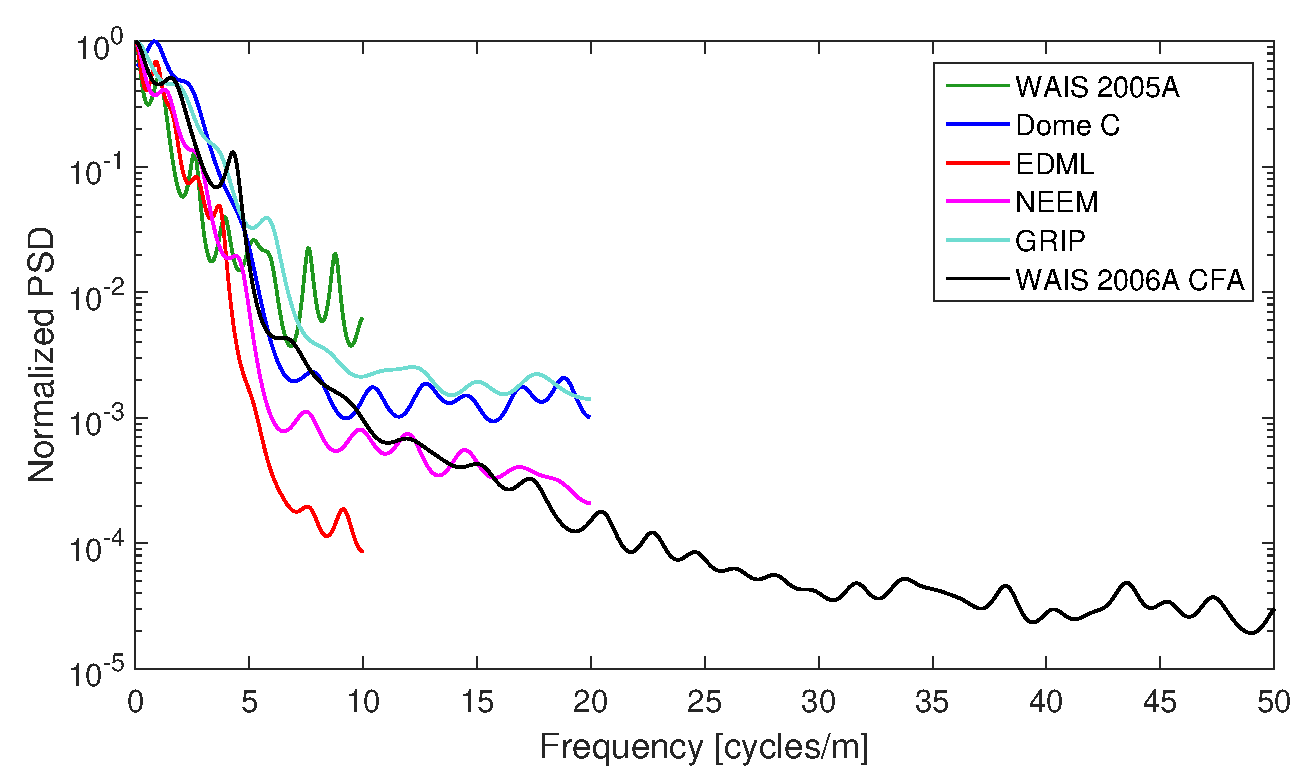
\includegraphics[width=0.9\linewidth]{PSD_discrete_plus_cfa_v1.eps}

	\end{minipage}%
	\begin{minipage}{0.5\textwidth}
		\centering
		\indent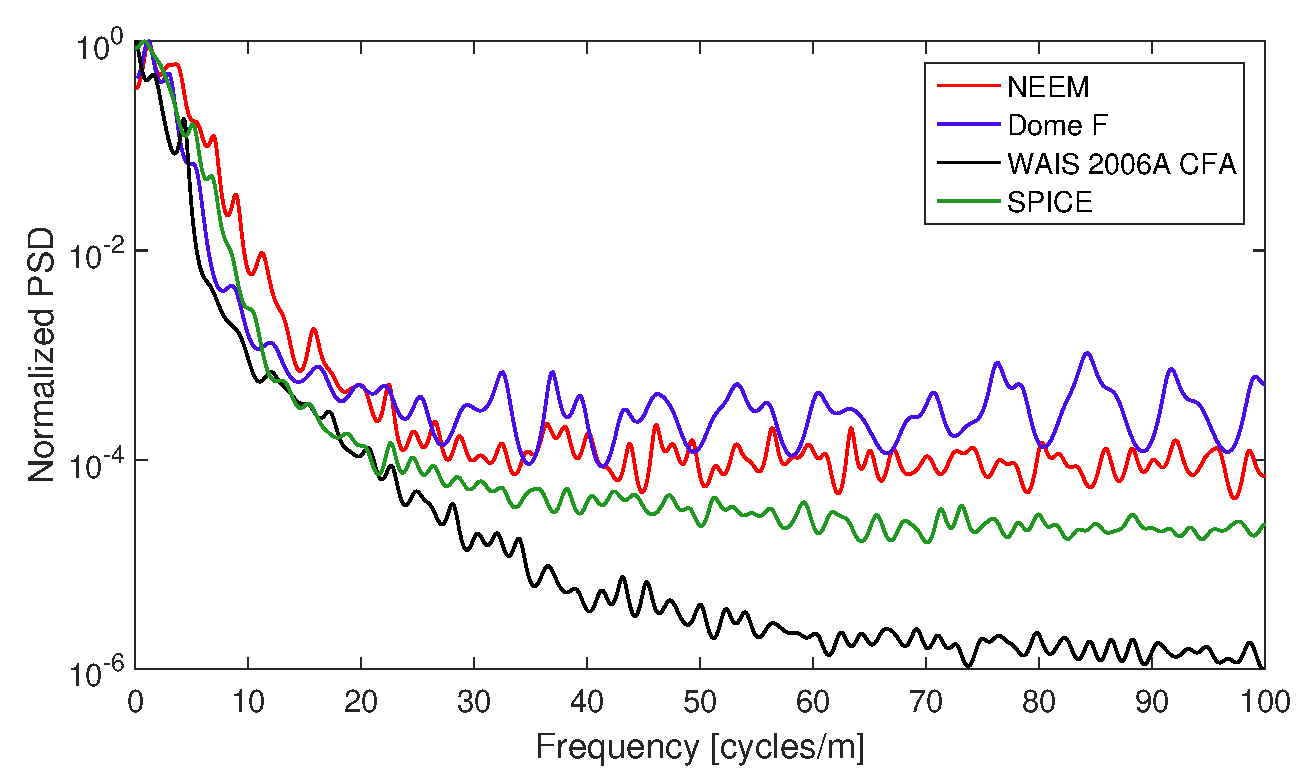
\includegraphics[width=0.9\linewidth]{PSD_CFA_v1.eps}

	\end{minipage}
	\caption{Left panel: The normalized PSD of five discretely measured $\delta^{18}$O series plotted together with the PSD of a $\delta^{18}$O WDC section. Right panel: The normalized PSD of four continuously measured $\delta$D series.}
\label{spectra_disVScfa}
\end{figure}

\begin{figure}
	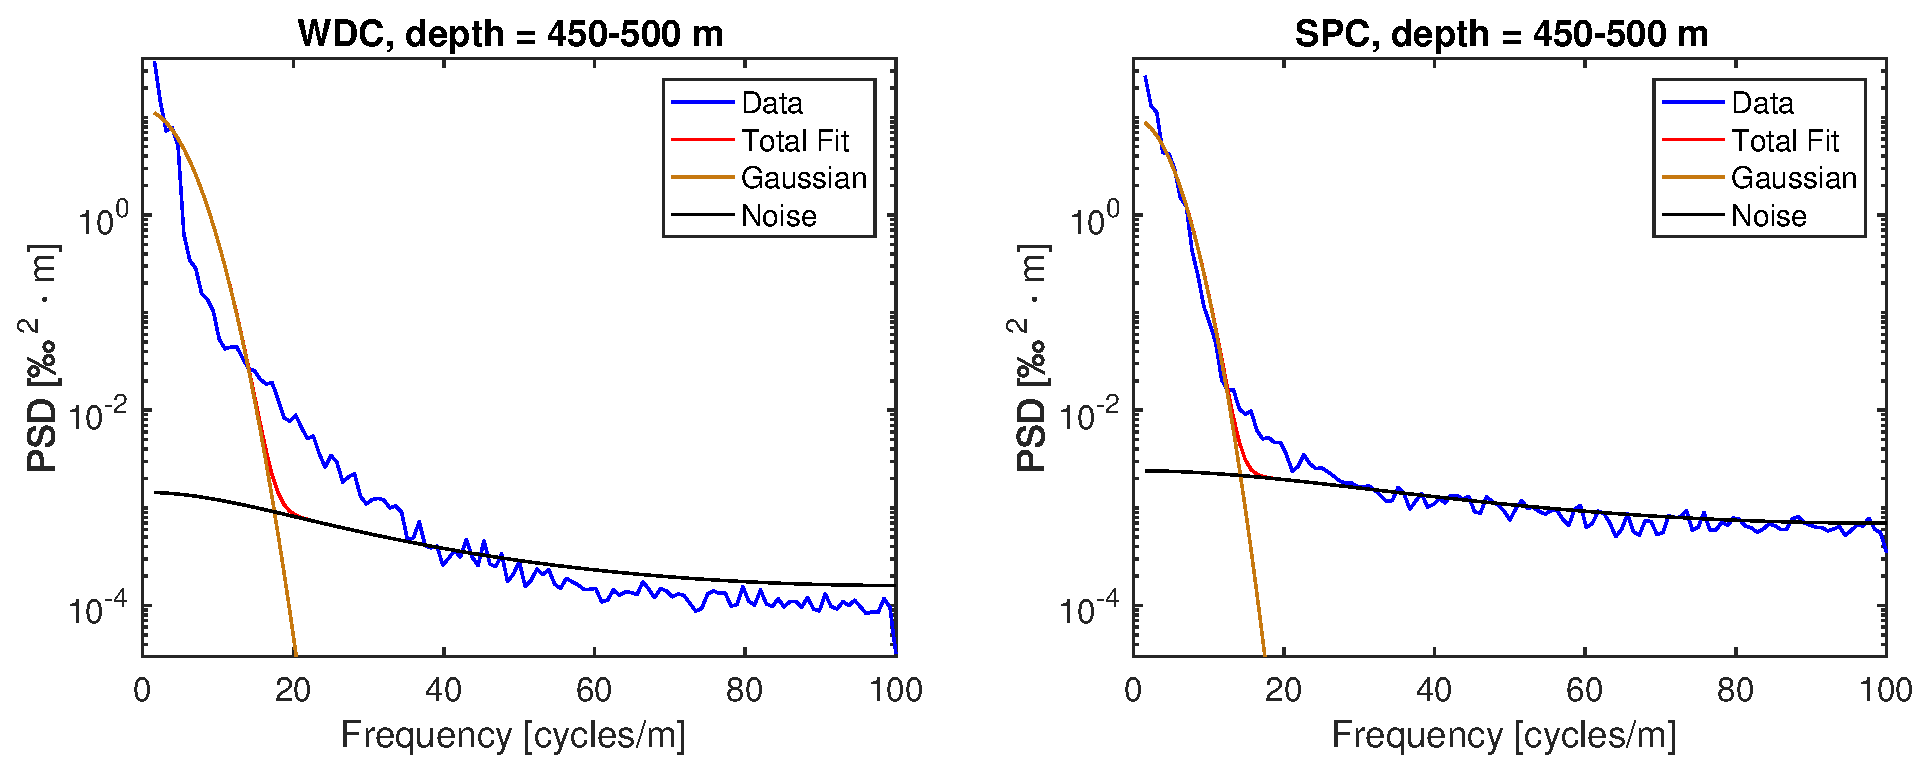
\includegraphics[width=\linewidth]{GR_fits.eps}
	\caption{Single-Gaussian multi-function fits for WDC and SPC at 450-500m depth. With only two functions, the parameterization is unable to effectively fit the entire data spectrum.} \label{GR_fits}
\end{figure}

\begin{figure}
	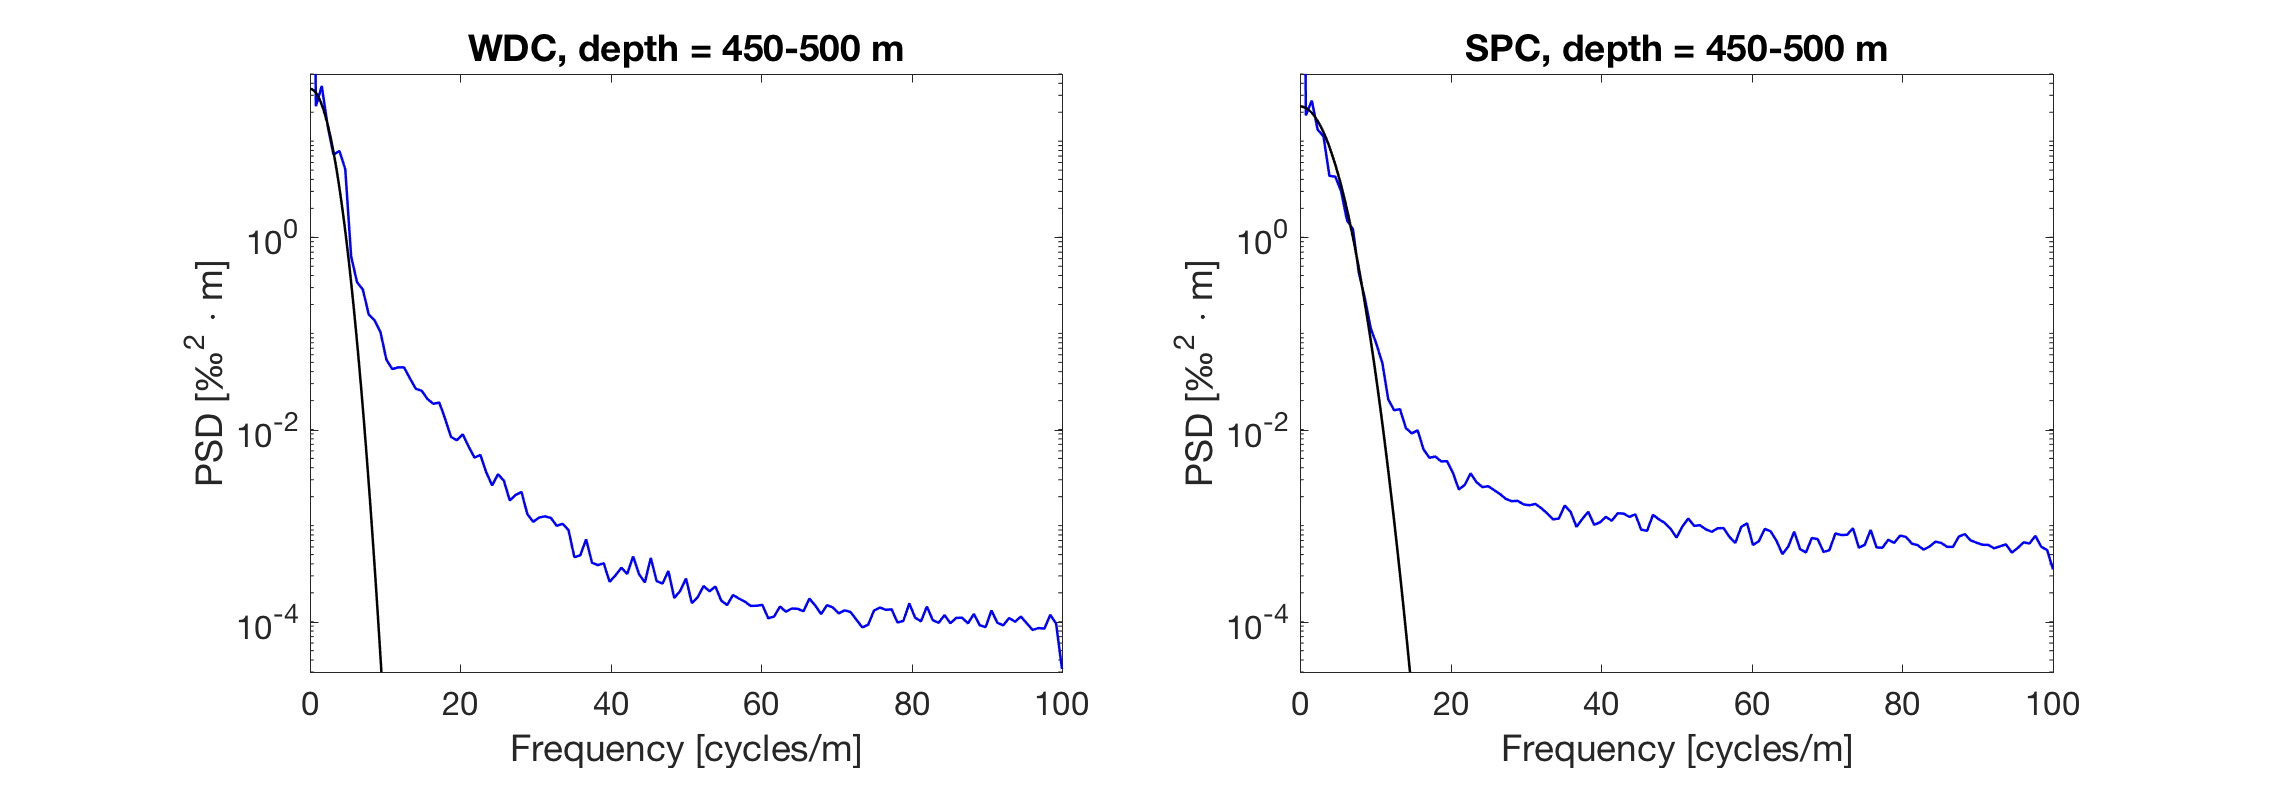
\includegraphics[width=\linewidth]{cutoff.eps}
	\caption{Cut-off technique on WDC and SPC at 450-500m depth. Blue curve is data spectrum and black curve is Gaussian fit.} \label{cutoff}
\end{figure}

\begin{figure}
	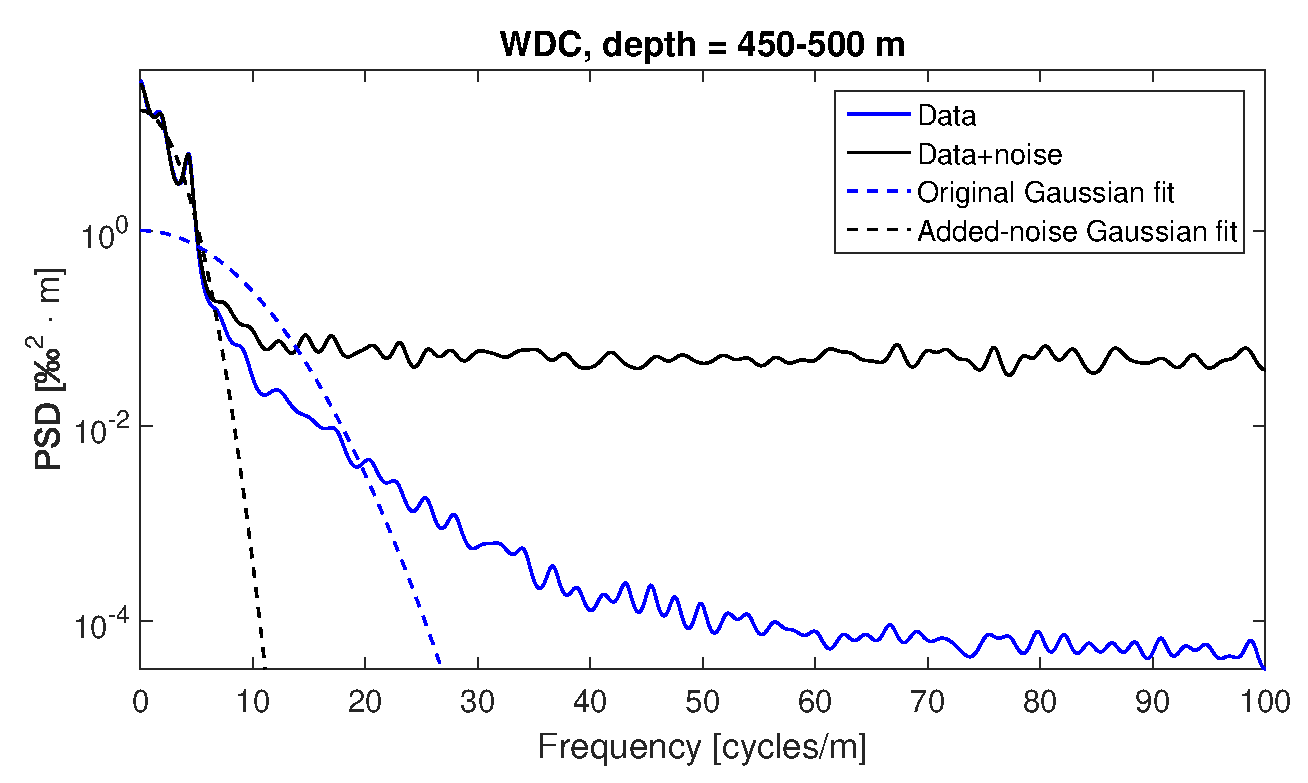
\includegraphics[width=.9\linewidth]{WAIS_spectrum_added_noise.eps}
	\caption{An illustration of the noise-adding technique for a $\delta$D section from WDC. The solid blue curve is the un-modified data and the black curve is data with noise added. The dashed lines represent the Gaussian functions fit using the two-function fitting technique. With the added noise, the dashed black model is able to effectively fit the data spectrum.} \label{WAIS_spectrum_added_noise}
\end{figure}

\begin{figure}
	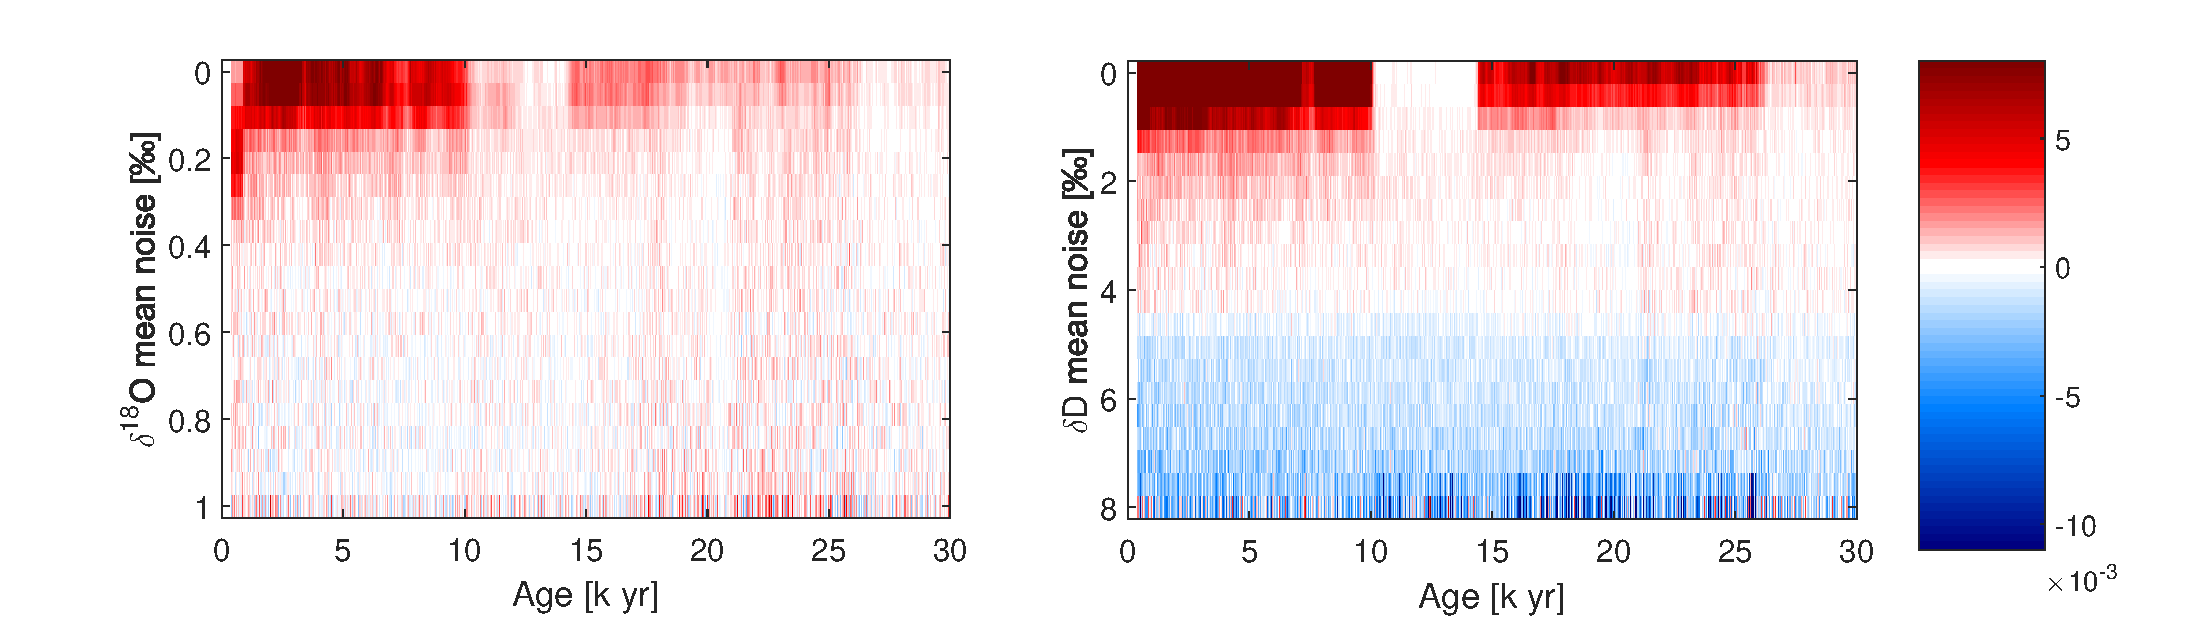
\includegraphics[width=\linewidth]{added_noise_sensitivity.eps}
	\caption{For WDC, the gradient of estimated diffusion lengths with respect to noise level plotted as a function of age. At each age, the lowest noise-level with a gradient of approximately zero is chosen as the optimal noise-level to be added.} \label{added_noise_sensitivity}
\end{figure}

\begin{figure}
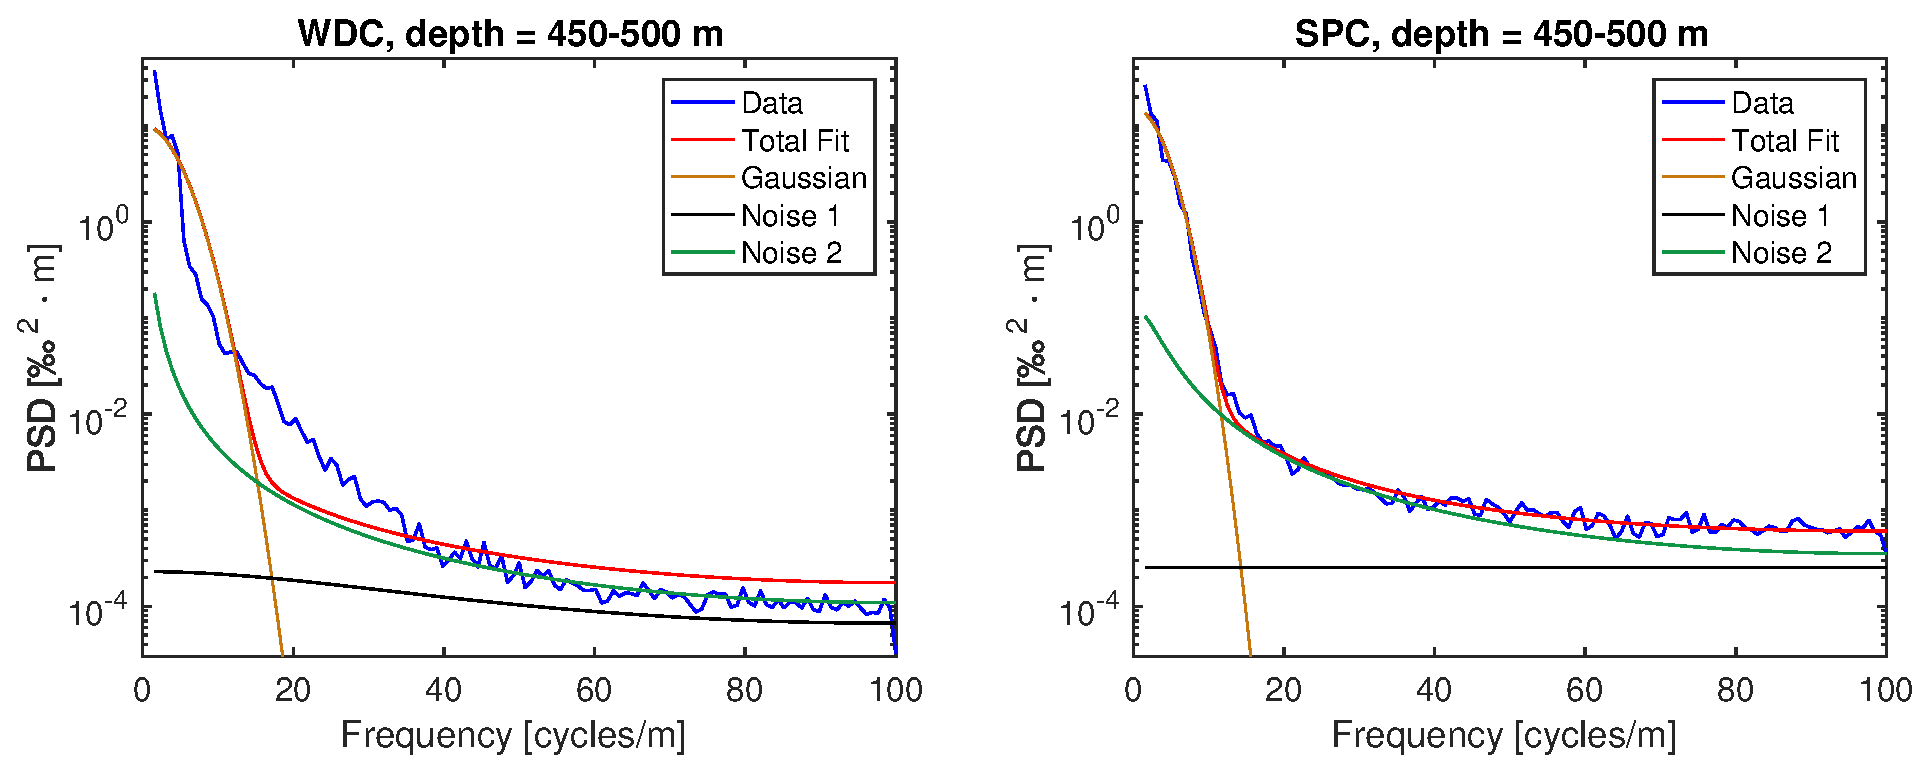
\includegraphics[width=.9\linewidth]{GRR_fits.eps}
\caption{Single Gaussian and two autoregressive-noise functions fit to WDC and SPC spectra.}\label{GRR_fits}
\end{figure}

\begin{figure}
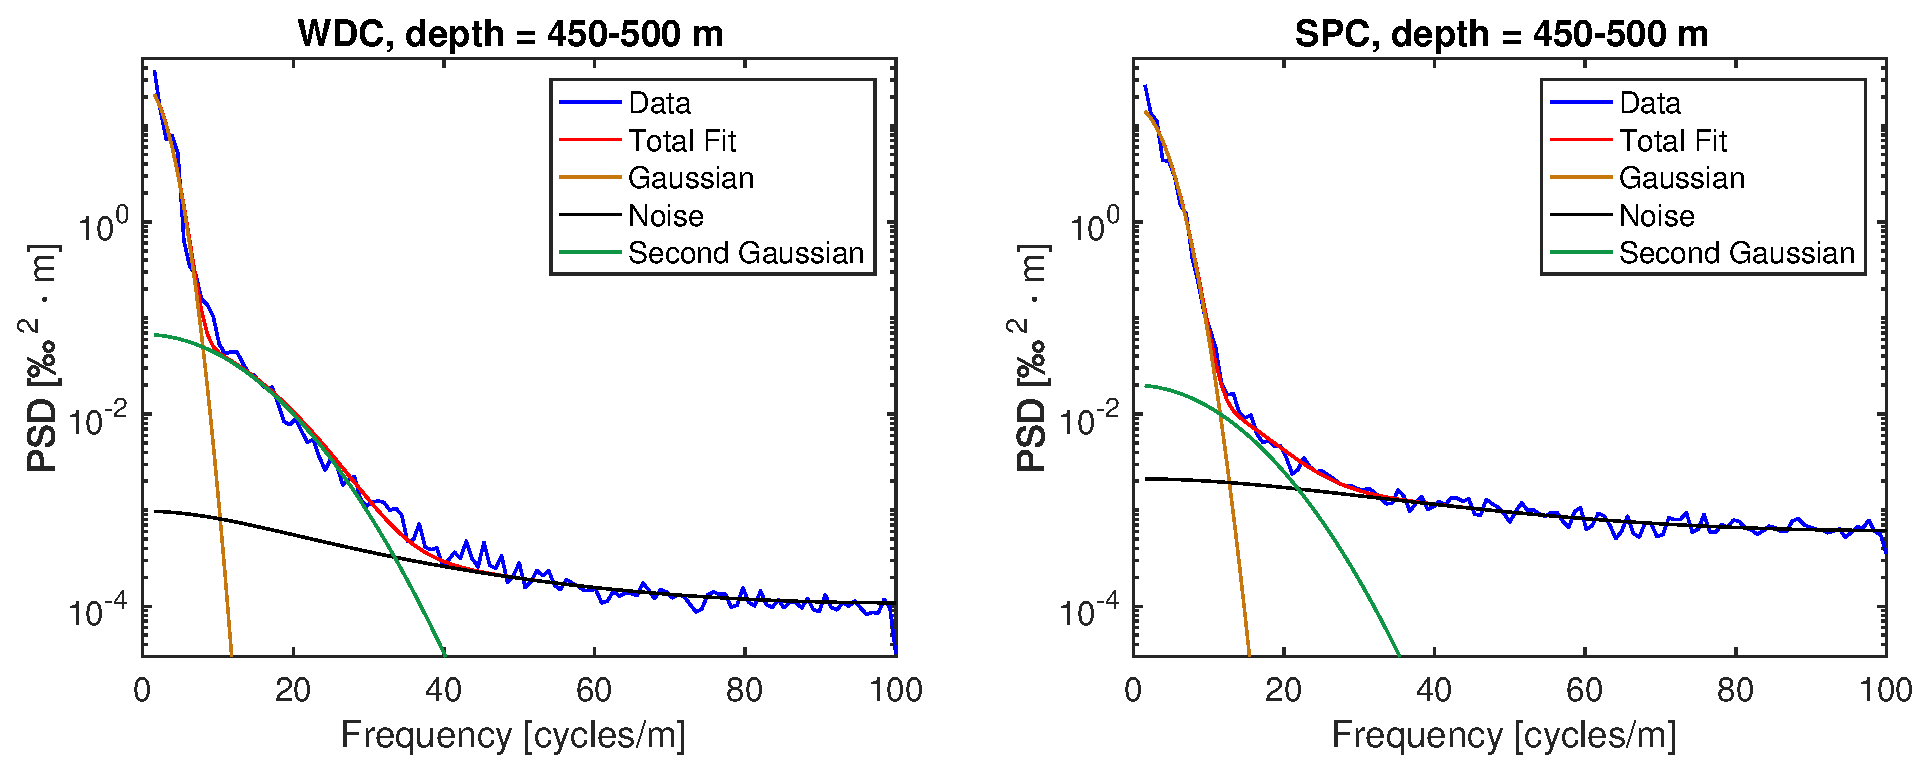
\includegraphics[width=.9\linewidth]{GGR_fits.eps}
\caption{Double-Gaussian multi-function technique fit to WDC and SPC spectra.}\label{GGR_fits}
\end{figure}

\begin{figure}
	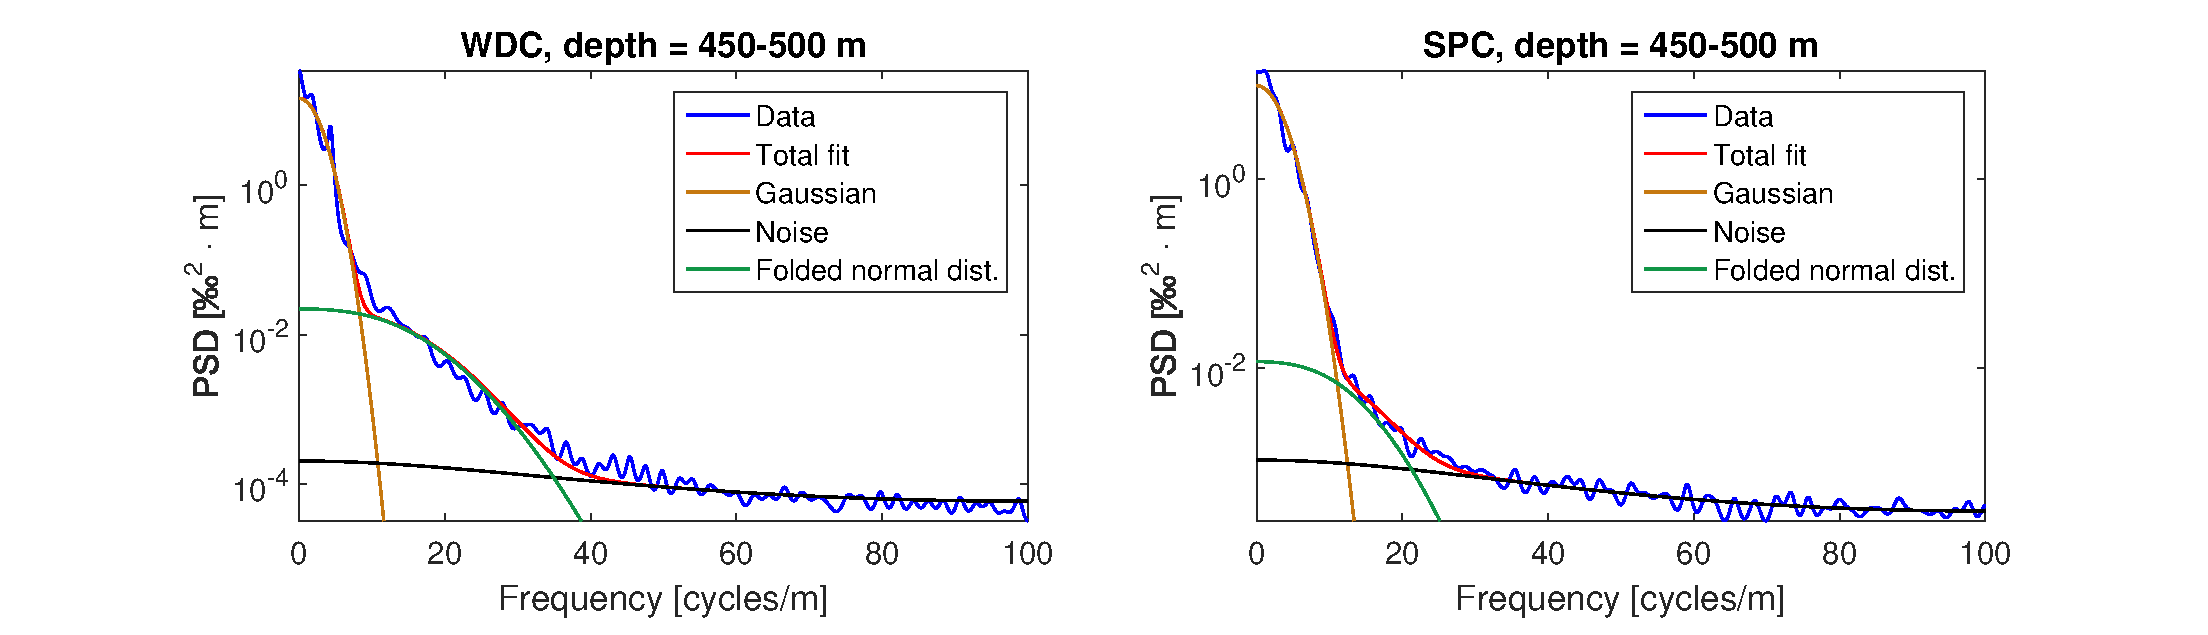
\includegraphics[width=1.1\linewidth]{folded_normal_gauss_spectrum.eps}
	\caption{Folded normal distribution multi-function technique fit to WDC and SPC spectra.}\label{folded_normal_gauss_spectrum}
\end{figure}

\begin{figure}
	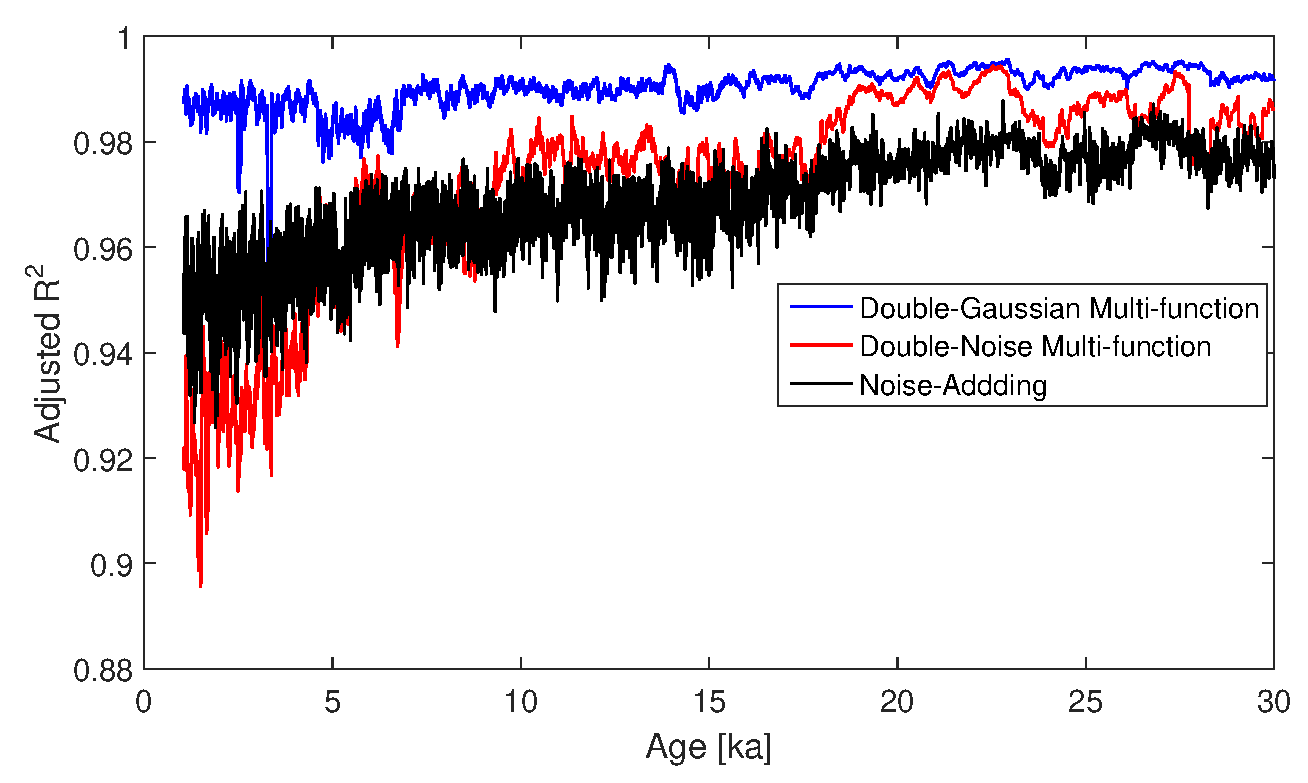
\includegraphics[width=.9\linewidth]{G_of_fit_1.eps}
	\caption{For WDC, the adjusted goodness of fit calculations through age for each fitting technique. FND results are identical to the results of a Gaussian curve and are not shown.} \label{G_of_fit_1}
\end{figure}

\begin{figure}
	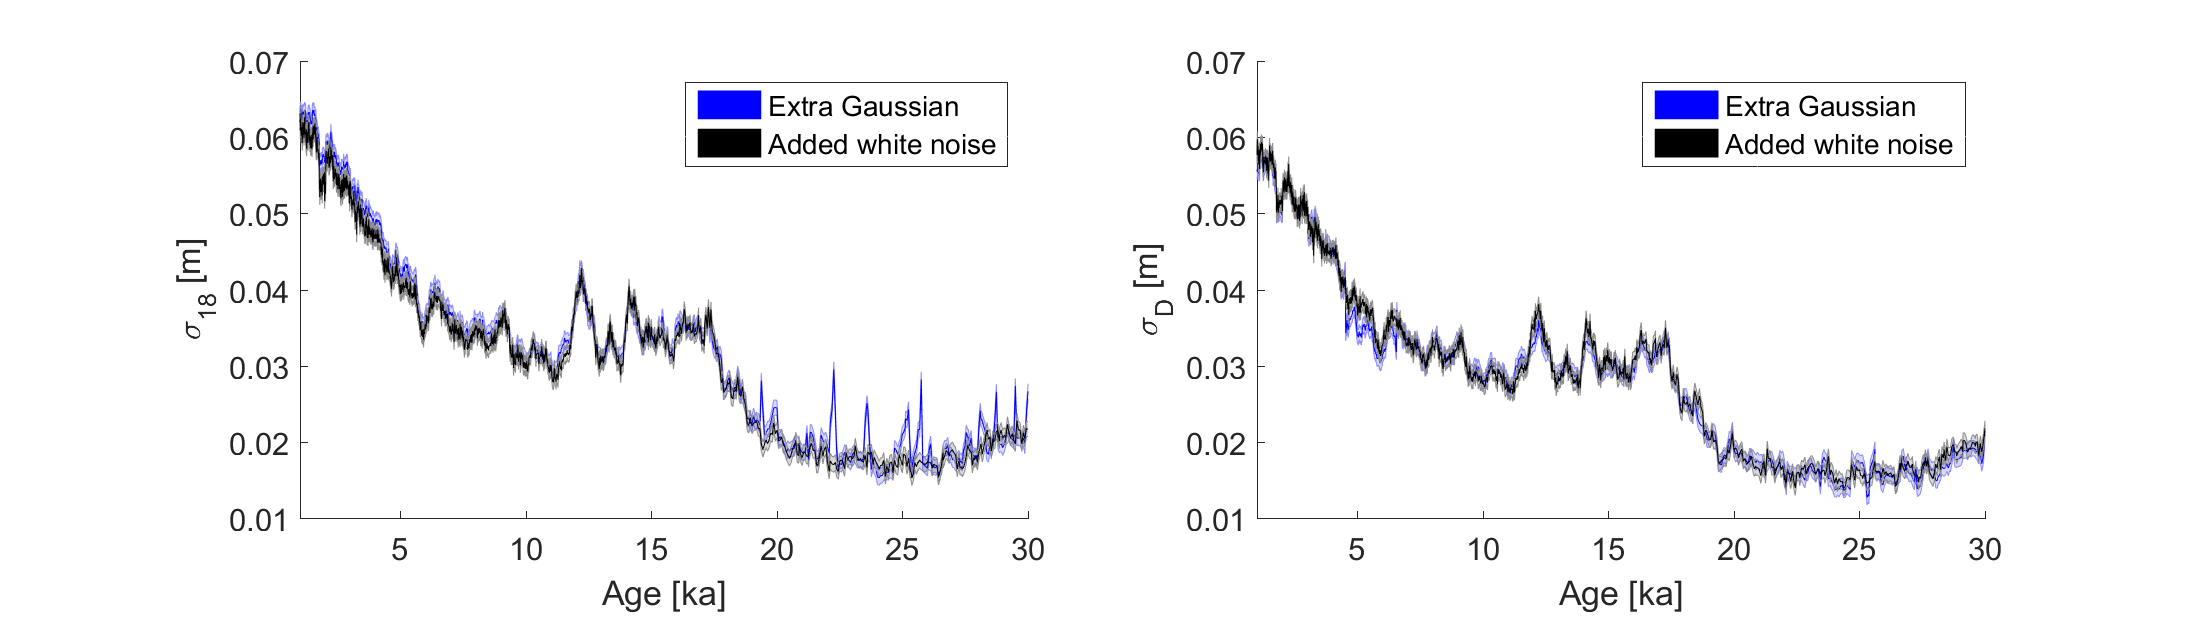
\includegraphics[width=\linewidth]{WAIS_diffusion_adding_noise.eps}
	\caption{WDC diffusion lengths of $\delta^{18}$O (left) and $\delta$D (right). Blue curve shows the multi-function Double-Gaussian technique, and the black curve shows the noise-adding technique.} \label{WAIS_diffusion_adding_noise}
\end{figure}

\begin{figure}
	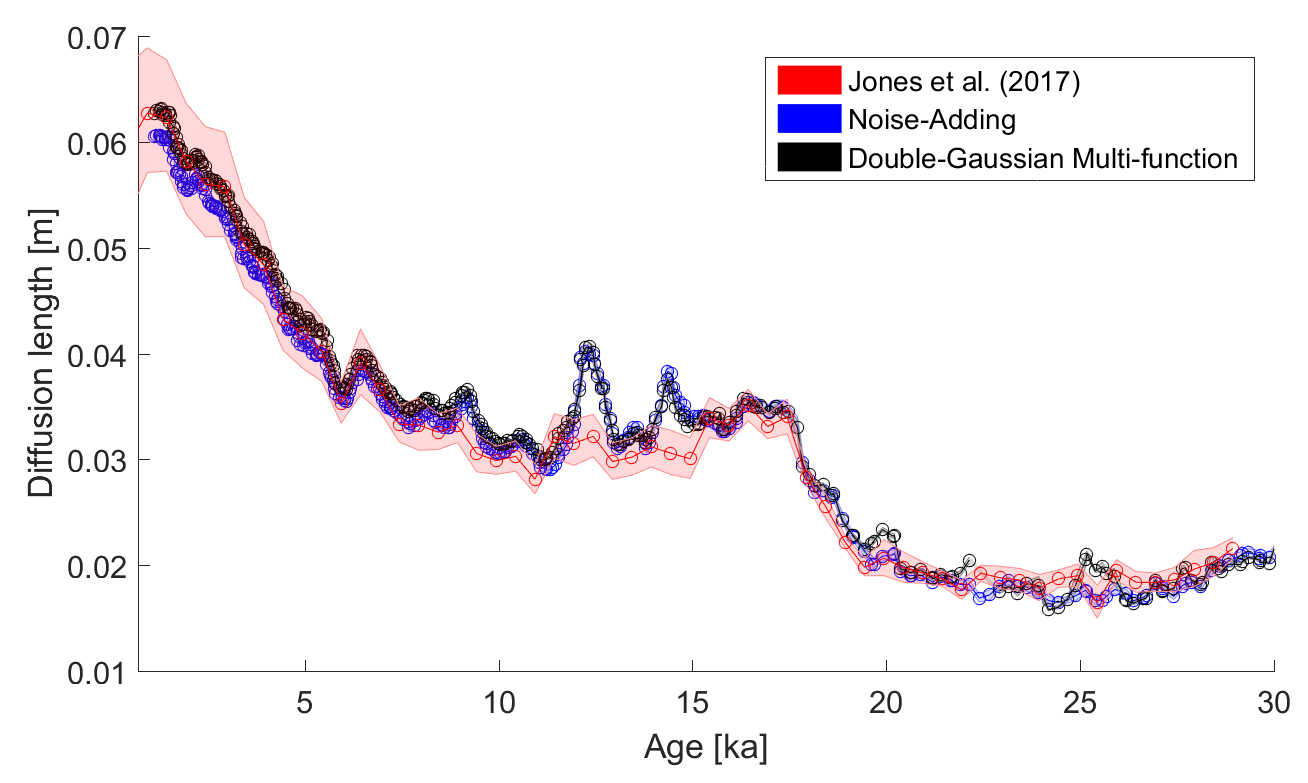
\includegraphics[width=.9\linewidth]{WAIS_diffusion_lengths.eps}
	\caption{Estimated WDC diffusion lengths of $\delta^{18}$O compared with those from \cite{Jones2017a}.} \label{WAIS_diffusion_lengths}
\end{figure}

\begin{figure}
	\includegraphics[width=.8\linewidth, angle =270]{smoothed_synthetic.pdf}
	\caption{Comparison of WDC power spectrum with that of synthetic ice core data with simulated CFA system smoothing.(Note: this is a screen shot from Christian's notes. We need a paper-ready version of this)} \label{smoothed_synthetic}
\end{figure}

\begin{figure}
	\includegraphics[width=.8\linewidth]{duplicate_spectra.eps}
	\caption{Power spectra from multiple measurements of the same depths of SPC from 1060m to 1075m. The blue curve shows the measurement from the original piece of ice. The red curve shows the measurement of a different sample from the same ice depth. The yellow curve shows the same data as the red, but with slightly different depths assigned to each data point.} \label{duplicate_spectra}
\end{figure}

\begin{table}
\caption{Summary of measurement specifications for each continuously measured core}
\label{tab:picarro_table}
\centering
\begin{tabular}{|c | c c c c|}
\hline
Core  & Picarro Instrument & Aquisition Rate & Melt Speed & Measurements Averaged \\
\hline
Dome F  & 1102 & 0.1 Hz & 3 cm/min & $\sim$1   \\
NEEM & 1102 (updated software) & 0.2 Hz & 3-4 cm/min & $\sim$2   \\
WDC & 2130 & 1.2 Hz & 2.5 cm/min & $\sim$14   \\
SPC & 2140 & 1.2 Hz & 2.25 cm/min & $\sim$15   \\
\hline
\end{tabular}
\end{table}

\end{document}

% Emma removed the following figure:
\begin{figure}
	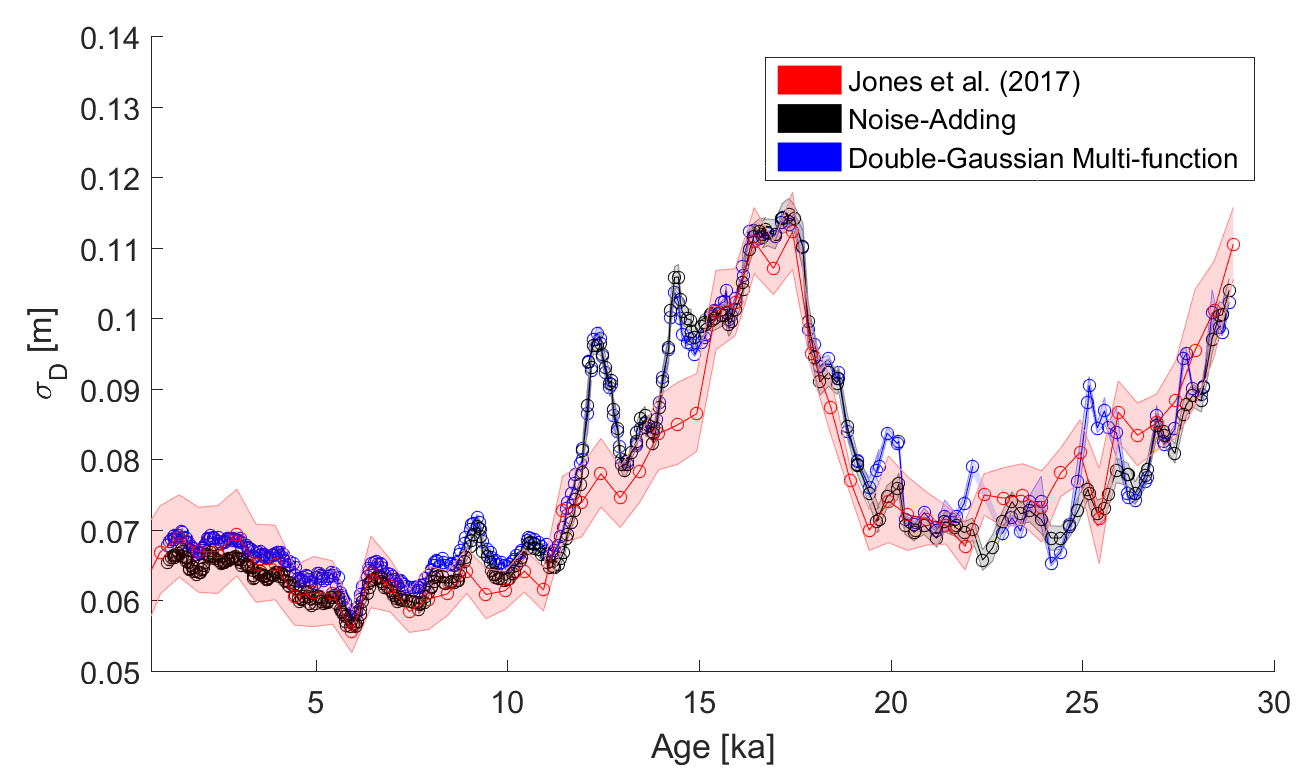
\includegraphics[width=.9\linewidth]{WAIS_diffusion_lengths_thinning_corr.eps}
	\caption{Thinning-corrected WDC diffusion lengths of $\delta^{18}$O compared with those from \cite{Jones2017a}.} \label{WAIS_diffusion_lengths_thinning_corr}
\end{figure}

%%%%%%%%%%%%%%%%%%%%%%%%%%%%%%%%%%%%%%%%%%%%%%%%%%%%%%%%%%%%%%%

More Information and Advice:

%% ------------------------------------------------------------------------ %%
%
%  SECTION HEADS
%
%% ------------------------------------------------------------------------ %%

% Capitalize the first letter of each word (except for
% prepositions, conjunctions, and articles that are
% three or fewer letters).

% AGU follows standard outline style; therefore, there cannot be a section 1 without
% a section 2, or a section 2.3.1 without a section 2.3.2.
% Please make sure your section numbers are balanced.
% ---------------
% Level 1 head
%
% Use the \section{} command to identify level 1 heads;
% type the appropriate head wording between the curly
% brackets, as shown below.
%
%An example:
%\section{Level 1 Head: Introduction}
%
% ---------------
% Level 2 head
%
% Use the \subsection{} command to identify level 2 heads.
%An example:
%\subsection{Level 2 Head}
%
% ---------------
% Level 3 head
%
% Use the \subsubsection{} command to identify level 3 heads
%An example:
%\subsubsection{Level 3 Head}
%
%---------------
% Level 4 head
%
% Use the \subsubsubsection{} command to identify level 3 heads
% An example:
%\subsubsubsection{Level 4 Head} An example.
%
%% ------------------------------------------------------------------------ %%
%
%  IN-TEXT LISTS
%
%% ------------------------------------------------------------------------ %%
%
% Do not use bulleted lists; enumerated lists are okay.
% \begin{enumerate}
% \item
% \item
% \item
% \end{enumerate}
%
%% ------------------------------------------------------------------------ %%
%
%  EQUATIONS
%
%% ------------------------------------------------------------------------ %%

% Single-line equations are centered.
% Equation arrays will appear left-aligned.

Math coded inside display math mode \[ ...\]
 will not be numbered, e.g.,:
 \[ x^2=y^2 + z^2\]

 Math coded inside \begin{equation} and \end{equation} will
 be automatically numbered, e.g.,:
 \begin{equation}
 x^2=y^2 + z^2
 \end{equation}

% IF YOU HAVE MULTI-LINE EQUATIONS, PLEASE
% BREAK THE EQUATIONS INTO TWO OR MORE LINES
% OF SINGLE COLUMN WIDTH (20 pc, 8.3 cm)
% using double backslashes (\\).

% To create multiline equations, use the
% \begin{eqnarray} and \end{eqnarray} environment
% as demonstrated below.
\begin{eqnarray}
  x_{1} & = & (x - x_{0}) \cos \Theta \nonumber \\
        && + (y - y_{0}) \sin \Theta  \nonumber \\
  y_{1} & = & -(x - x_{0}) \sin \Theta \nonumber \\
        && + (y - y_{0}) \cos \Theta.
\end{eqnarray}

%If you don't want an equation number, use the star form:
%\begin{eqnarray*}...\end{eqnarray*}

% Break each line at a sign of operation
% (+, -, etc.) if possible, with the sign of operation
% on the new line.

% Indent second and subsequent lines to align with the first character following the equal sign on the first line.

% Use an \hspace{} command to insert horizontal space into your equation if necessary. Place an appropriate unit of measure between the curly braces, e.g. \hspace{1in}; you may have to experiment to achieve the correct amount of space.


%% ------------------------------------------------------------------------ %%
%
%  EQUATION NUMBERING: COUNTER
%
%% ------------------------------------------------------------------------ %%

% You may change equation numbering by resetting
% the equation counter or by explicitly numbering
% an equation.

% To explicitly number an equation, type \eqnum{}
% (with the desired number between the brackets)
% after the \begin{equation} or \begin{eqnarray}
% command.  The \eqnum{} command will affect only
% the equation it appears with; LaTeX will number
% any equations appearing later in the manuscript
% according to the equation counter.
%

% If you have a multiline equation that needs only
% one equation number, use a \nonumber command in
% front of the double backslashes (\\) as shown in
% the multiline equation above.

%% ------------------------------------------------------------------------ %%
%
%  SIDEWAYS FIGURE AND TABLE EXAMPLES
%
%% ------------------------------------------------------------------------ %%
%
% For tables and figures, add \usepackage{rotating} to the paper and add the rotating.sty file to the folder.
% AGU prefers the use of {sidewaystable} over {landscapetable} as it causes fewer problems.
%
% \begin{sidewaysfigure}
% \includegraphics[width=20pc]{samplefigure.eps}
% \caption{caption here}
% \label{label_here}
% \end{sidewaysfigure}
%
% \begin{sidewaystable}
% \caption{}
% \begin{tabular}
% Table layout here.
% \end{tabular}
% \end{sidewaystable}
